\documentclass[conference]{sig-alternate-10pt}
\usepackage{palatino}
\usepackage{fancyhdr}
\usepackage{color}
\usepackage{graphicx}
\usepackage{epsfig}
\usepackage[normalem]{ulem}
\usepackage{epsf}
% \usepackage{subfigure}
\usepackage{latexsym}
\usepackage{url}
\usepackage{amsmath}
\usepackage{multirow}
\usepackage{times}
\usepackage{alltt}
\usepackage{xspace}
\usepackage{listings}
\usepackage{amsfonts}
\usepackage{mathtools}
\usepackage{fancyref}
\pagestyle{plain}
\usepackage{multicol}
\usepackage{wrapfig}
\usepackage{tabularx}
\usepackage{caption}
\usepackage{subcaption}
\usepackage{hyphenat}

\widowpenalty=0
\clubpenalty=0

\pdfpagewidth=8.5 true in
\pdfpageheight=11 true in

\setlength{\tabcolsep}{3pt}

\newcommand{\todo}{\textbf{\textcolor{red}{more here ... }}}

\newcommand{\rephrase}{\vspace{+1.5mm} \noindent
  \textbf{\large{\textcolor{red}{re-phrase, re-organize the following.}}}}

\newcommand{\shrinkhdr}{\vspace{-1mm}}  
\newcommand{\shrinkhdrafter}{\vspace{-1mm}} 

\newenvironment{compactList}{\begin{list}{$\bullet$}{\leftmargin=0.5em}
    {   \setlength{\itemsep}{0mm}
        \setlength{\topsep}{0mm}
        \setlength{\partopsep}{0mm}}
    }
{\end{list}}

\newcounter{foo}
\newenvironment{myenumerate}{\begin{list}{\arabic{foo}.}{ 
        \usecounter{foo}
        \setlength{\topsep}{0mm}
        \setlength{\itemsep}{0mm}
}}{ \end{list}
}

\newcommand{\Paragraph}[1]{\vspace{+1.5mm} \noindent \textbf{#1}}
\newcommand{\subparagraph}[1]{\vspace{+1mm} \noindent \textit{#1}}

% \newcommand{\Quote2}[1]{
%   \vspace{+1mm} \begin{changemargin}{0.5cm}{0.5cm}\textit{#1}\end{changemargin}
%   \vspace{+1mm} }
\newcommand{\alert}[1]{\textbf{\textcolor{red}{#1}}}

\newcommand{\Quote}[1]{\vspace{+1mm} \textit{#1} \vspace{+1mm}}  
\newcommand{\Subsubsection}[1]{\shrinkhdr\shrinkhdr\subsubsection{#1}\shrinkhdrafter}
\newcommand{\SubsubsectionS}[1]{\shrinkhdr\subsubsection*{#1}\shrinkhdrafter}
\newcommand{\Subsection}[1]{\shrinkhdr\subsection{#1}\shrinkhdrafter}
\newcommand{\Section}[1]{\shrinkhdr\section{#1}\shrinkhdrafter} 
\newcommand{\SectionS}[1]{\shrinkhdr\shrinkhdr\section*{#1}\shrinkhdrafter}

\newtheorem{thm}{Theorem}
\newtheorem{cor}[thm]{Corollary}

% \newenvironment{proof}{\noindent{\bf Proof (Sketch):}\hspace*{0.5em}}% {\hspace*{\fill}\qed} 

\newcommand{\Succ}[1]{\ensuremath{\mathrm{\Gamma}^{\mathord{+}}(#1)}}
\newcommand{\Pred}[1]{\ensuremath{\mathrm{\Gamma}^{\mathord{-}}(#1)}}

\newcommand{\prewrite}[3]{\ensuremath{{#1}[{#2}\mapsto{#3}]}}

% Try to fill figures onto the page
\newcommand{\ns}{\mbox{ns-3}\xspace}
\newcommand{\goodgadget}{{\sc GoodGadget}\xspace}
\newcommand{\goodgadgets}{{\sc GoodGadgets}\xspace}
\newcommand{\badgadget}{{\sc BadGadget}\xspace}
\newcommand{\disagree}{{\sc Disagree}\xspace}
\newcommand{\pv}{{\sc PathVector}\xspace}
\newcommand{\HLP}{{\sc HLP}\xspace}

\newcommand{\theHalgorithm}{\arabic{algorithm}}
\renewcommand{\topfraction}{1.00}
\renewcommand{\floatpagefraction}{1.00}
\renewcommand{\textfraction}{0.00}
\renewcommand{\dbltopfraction}{1.00}
\renewcommand{\dblfloatpagefraction}{1.00}

\def\ttt{~}
\def\mc{\prec_{mc}}
\def\po{\prec}
%\def\domain{\cal D}
\def\fc#1#2#3{#1 \mkern1mu\hbox{:}\; #2 \leadsto #3}
\def\mci#1#2#3{#1 \mkern1mu\hbox{:}\; #2 \prec_{mc} #3}
\def\eci#1#2#3{#1 \mkern1mu\hbox{:}\; #2 =_{ec} #3}
\def\Xvec{{\vec X}}
\def\Yvec{{\vec Y}}
\def\xvec{{\vec x}}
\def\yvec{{\vec y}}
\def\imp{\mathrel{:}\mathrel{-}}
\def\dcone{\bigvee_{i=1}^n {\cal C}_i}
\def\dctwo{\bigvee_{i=1}^m {\cal B}_i}
\def\edb{e_1,\ldots,e_m}
\def\comp{\circ}
\newcommand{\calp}{\ensuremath{\mathcal{P}}}
\newcommand{\calf}{\ensuremath{\mathcal{F}}}
\newcommand{\calc}{\ensuremath{\mathcal{C}}}
\newcommand{\caln}{\ensuremath{\mathcal{N}}}
\newcommand{\call}{\ensuremath{\mathcal{L}}}
\newcommand{\cala}{\ensuremath{\mathcal{A}}}
\newcommand{\calr}{\ensuremath{\mathcal{R}}}
\newcommand{\calv}{\ensuremath{\mathcal{V}}}
\newcommand{\calq}{\ensuremath{\mathcal{Q}}}
\newcommand{\calm}{\ensuremath{\mathcal{M}}}
%\newcommand{\tukwila}{\mbox{\sf Tukwila}}
\newcommand{\tukwila}{Tukwila}
%\newcommand{\Tukwila}{\mbox{\sf Tukwila}}
\newcommand{\Tukwila}{Tukwila}
\newcommand{\calo}{\ensuremath{\mathcal{O}}}
\newcommand{\calw}{\ensuremath{\mathcal{W}}}
\newcommand{\cals}{\ensuremath{\mathcal{S}}}
\newcommand{\calt}{\ensuremath{\mathcal{T}}}
\newcommand{\cale}{\ensuremath{\mathcal{E}}}
\newcommand{\cali}{\ensuremath{\mathcal{I}}}
\newcommand{\cald}{\ensuremath{\mathcal{D}}}
\newcommand{\calg}{\ensuremath{\mathcal{G}}}
\newif\iffullpaper
%\fullpaperfalse
\fullpapertrue


\newcommand{\ojoin}{\mbox{}^-_-\!\raisebox{-0.3mm}{$\bowtie$}\!^-_-}



%%%%%%%%%%%%%%%%  Weld's additions

\newcommand{\comment}[1]{}
\newcommand{\NOTE}[1]{\marginpar{\em {#1}}}
\newcommand{\bug}
    {\mbox{\rule{2mm}{2mm}}}
\newcommand{\Bug}[1]
    {\bug \footnote{BUG: {#1}}}
\newcommand{\TT}[1]{\mbox{\tt #1}}
\newcommand{\bi}{\begin{itemize}}
\newcommand{\ei}{\end{itemize}}
\newcommand{\BE}{\begin{enumerate}}
\newcommand{\EE}{\end{enumerate}}
\newcommand{\link}[1]{\url{#1}}


%\newcommand{\etc}{\mbox{\it etc.}}
%\newcommand{\eg}{\mbox{\it e.g.}}
%\newcommand{\ie}{\mbox{\it i.e.}}
%\newcommand{\Eg}{\mbox{\it E.g.}}
%\newcommand{\Ie}{\mbox{\it I.e.}}
\newcommand{\etc}{\mbox{etc}\xspace}
\newcommand{\eg}{\mbox{e.g.,}\xspace}
\newcommand{\ie}{\mbox{i.e.}\xspace}
\newcommand{\Eg}{\mbox{E.g.,}\xspace}
\newcommand{\Ie}{\mbox{I.e.}}
\newcommand{\?}{\mbox{?}}

\newcommand{\tuple}[1]
        {\mbox{$\langle{#1}\rangle$}}
\newcommand{\set}[1]
        {\mbox{$\{{#1}\}$}}
\newcommand{\size}[1]{\mbox{$\mid\!#1\!\mid$}}
\newcommand{\fun}[2]{$\mathbf{#1}(#2)$}

\newtheorem{defn}{Definition}
\newtheorem{them}{Proposition}          
% \newtheorem{lemma}[them]{Proposition}
% \newtheorem{example}{Example}
% \newtheorem{ex}{Example}%[section]



%%%%%%%%%%%%%%%%%% Friedman's additions

%\newcommand{\myps}[3]{\psfig{figure=#1,scale=100*{#2}}}
\newcommand{\myps}[3]{\rotatebox{#3}{\scalebox{#2}{\includegraphics{#1}}}}

%\newcommand{\myitem}[1] {{\noindent}{\bf {#1}}}
\newcommand{\myitem}[1] {\item {#1}}
\newcommand{\mylist}{\begin{itemize_squeeze}}
\newcommand{\mylistend}{\end{itemize_squeeze}}
\newcommand{\myparagraph}[1]{\vspace{-.15in}\paragraph{#1}}
\newcommand{\mysubsection}[1]{\vspace{-.1in}\subsection{#1}\vspace{-.12in}}
\newcommand{\mysubsubsection}[1]{\vspace{-.1in}\subsubsection{#1}\vspace{-.12in}}
\newcommand{\mysubsubsections}[1]{\vspace{-.1in}\subsubsection*{#1}\vspace{-.12in}}
\newcommand{\mycaption}[1]{\vspace{-.1in}\caption{#1}\vspace{-.13in}}
\newcommand{\mysection}[1]{\vspace{-.15in}\section{#1}\vspace{-.15in}}
%\newcommand{\pair}[2]   {\mbox{$\langle{\mbox{#1}},{\mbox{#2}}\rangle$}}
%\newcommand{\tuple}[1]   {\mbox{$\langle{\mbox{#1}}\rangle$}}
\newcommand{\triple}[3]{\ensuremath{(#1,#2,#3)}}
\newcommand{\pair}[2]{\ensuremath{(#1,#2)}}
\newcommand{\constant}[1]{\mbox{$\tt{#1}$}}
\newcommand{\etal}       {{\em et al.\/}}
\newcommand{\naive}      {na\"{\i}ve\xspace}
\newcommand{\Naive}      {Na\"{\i}ve}
\newcommand{\new}[1]{{\em #1\/}}                % New term (emphasized).
%\newcommand{\new}[1]     {\emph{#1}}
%\newcommand{\fixedfont}[1] {\texttt{#1}}
\newcommand{\fixedfont}[1]{#1} % fix this

\newenvironment{itemize_squeeze}{
  \begin{list}{$\bullet$}{
                \setlength{\rightmargin}{0pt}% Horizontal spacing
                \setlength{\listparindent}{0pt}
                \setlength{\itemindent}{0pt}
                \setlength{\labelwidth}{5pt}
                \setlength{\labelsep}{3pt}
                \setlength{\leftmargin}{8pt}
                \setlength{\parsep}{0pt}%        Vertical spacing
                \setlength{\itemsep}{0pt}
                \setlength{\topsep}{3pt}
                \setlength{\parskip}{0pt}
                \setlength{\partopsep}{0pt}}}
{
%                \addtolength{\textwidth}{1in}%               Misc
%                \addtolength{\oddsidemargin}{-.5in}
%                \addtolength{\textheight}{1.5in}
%                \addtolength{\topmargin}{-1in}
  \end{list}}

\newenvironment{itemize_squeeze_oneitem}{
  \begin{list}{ }{
                \setlength{\rightmargin}{0pt}% Horizontal spacing
                \setlength{\listparindent}{0pt}
                \setlength{\itemindent}{0pt}
                \setlength{\labelwidth}{5pt}
                \setlength{\labelsep}{3pt}
                \setlength{\leftmargin}{8pt}
                \setlength{\parsep}{0pt}%        Vertical spacing
                \setlength{\itemsep}{0pt}
                \setlength{\topsep}{3pt}
                \setlength{\parskip}{0pt}
                \setlength{\partopsep}{0pt}}}
{
  \end{list}}


%%%%%%%% Macros for examples, zives:
% \begin{example}{width}..\end{example} environment establishes minipage, 
%       increments ex. counter
% \begin{ecolumn}{width} creates a column with small font
%
% \ecaption{name}{text} creates a counter label plus a caption
% \eref{name} returns the counter value
% \newcounter{example}
% \newenvironment{example}[1][\textwidth]{\begin{minipage}[t]{#1}\addtocounter{example}{1}}{\end{minipage}}
\newenvironment{ecolumn}[1][3.5in]{\begin{minipage}[t]{#1}\footnotesize}{\end{minipage}}
\newcommand{\eref}[1]{\arabic{ex:#1}}
\newcommand{\ecaption}[2]{\center{Example \arabic{example}: #2}\vspace{+0.15in}\newcounter{ex:#1}\setcounter{ex:#1}{\arabic{example}}}

% Outputs a figure with a divider line at the top and bottom
\newenvironment{linedfig}{\begin{figure*}[tb]\rule{\textwidth}{0.5pt}}{\rule{\textwidth}{0.5pt}\end{figure*}}

% Use \openbox{\newcommandname} and \closebox{\newcommandname} (where \newcommandname is
% a command name you invent) to create a framed box into which you can put verbatim, etc.
% You can nest this inside of a figure environment, also (but the caption goes *outside*).
% \newcommand{\openbox}[1]{\newsavebox{#1}\begin{lrbox}{#1}}
\newcommand{\closebox}[1]{\end{lrbox}\fbox{\usebox{#1}}}

\newcommand{\id}{{\tt ID}}
\newcommand{\idref}{{\tt IDREF}}
\newcommand{\idrefs}{{\tt IDREFS}}
\newcommand{\pcdata}{{\tt PCDATA}}

\newcommand{\appearedin}[1] {
\vspace{-2.5in}
\vbox to 0pt{\hfill\framebox{\bf \it Appeared in proceedings of #1}}
\vspace{2.5in}
}

\newcommand{\submittedto}[1] {
\vspace{-2.5in}
\vbox to 0pt{\hfill\framebox{\bf \it Submitted to #1}}
\vspace{2.5in}
}

\newenvironment{example2}{\begin{ex} \nopagebreak
  \begin{rm}}{{\hfill$\Box$}\end{rm}\end{ex}} 

% \newenvironment{theorem}{\begin{thm} \nopagebreak}{\end{thm}}

\newenvironment{proof2}{\noindent {\bf Proof. } \nopagebreak 
\begin{normalsize}}{\end{normalsize}{\hfill$\Box$}\vspace*{0.2cm}}

% \newenvironment{definition}[1]{\begin{defin}\begin{rm}({\bf 
% #1})}{{\hfill$\Box$}\end{rm}\end{defin}}

\newenvironment{examp}{\begin{ex} \nopagebreak
  \begin{rm}}{{\hfill$\Box$}\end{rm}\end{ex}} 

% \newenvironment{corollary}{\begin{corol} \nopagebreak}{\end{corol}}

\newenvironment{namedproof}[1]{\noindent {\bf Proof.}~(#1) \nopagebreak
\begin{normalsize}}{\end{normalsize}{\hfill$\Box$}\vspace*{0.2cm}}

\def\papernumber #1 raised #2 {
%\vspace{-#2}
\vbox to 0pt{\hfill\framebox{\bf \it Paper \# #1}}
\vspace{#2}
}

\def\dand{{\mbox{$\; \& \;$}}}
\def\dif{{\mbox{$\; :- \;$}}}
\def\tand{{\mbox{$\; \sqcap \;$}}}

\def\classic{{\sc Classic}}

\newcommand{\V}{\mbox{${\cal V}$}}
\newcommand{\R}{\mbox{${\cal R}$}}
\newcommand{\barX}{{\bar X}}
\newcommand{\barY}{{\bar Y}}
\newcommand{\barA}{{\bar A}}
\newcommand{\barC}{{\bar C}}
\newcommand{\plan}{{\cal P}}
\newcommand{\query}{{\cal Q}}
\newcommand{\viewdef}{{\cal V}}
\newcommand{\vlit}{v}
\newcommand{\marker}{\star}
%\newcommand{\system}{``Q''}
\newcommand{\system}{Tukwila-CQP}

\newcommand{\eat}[1]{}

\newcommand{\reminder}[1]{{\bf  [[  #1 ]]}\typeout{#1}}
%\newcommand{\reminder}[1]{{\bf  [[  #1 ]]}\typeout{}}

\newtheorem{Def}{Definition}
\newtheorem{Not}{Notation}
\newtheorem{Claim}{Claim}
\newtheorem{Theorem}{Theorem}
\newtheorem{Lem}{Lemma}
\newtheorem{Cor}{Corollary}
\newtheorem{Example}{Example}
\newtheorem{Assumption}{Assumption}
\newtheorem{Constraint}{Constraint}

% \def\Dlog{{\em NDlog}\xspace}
% \def\Mlog{{\em Mozlog}\xspace}
% \def\Lang{{\em SeNDlog}\xspace}
% \def\P2{{\em P2}\xspace}
% \def\Pitu{{\em P2}\xspace}
% \def\SIVD{{\em SIV-divide}\xspace}
% \def\SVI{{\em SVI}\xspace}
% \def\VSI{{\em VSI}\xspace}
% \def\DSys{{\em DeNS}\xspace}
% \def\MSys{{\em Mosaic}\xspace}
% \def\VSys{{\em DNV}\xspace}
% \def\Views{{\em CViews}\xspace}
% \def\View{{\em CView}\xspace}
% \def\FVN{{\em FVN}\xspace}
% \def\FVR{{\em FVR}\xspace}
\def\Sys{{\em DBN}\xspace} % Database-based Networking
\newenvironment{SQL}{\begin{alltt}\footnotesize}{\end{alltt}}
\newenvironment{NDlog}{\vspace{-1mm}\begin{alltt}\scriptsize}{\end{alltt}\vspace{-1mm}}
\newcommand{\datalogspace}{\textcolor[gray]{1}{.}\hspace{0.8in}}
\newcommand{\lab}[1]{\textrm{\bf #1:\hspace{0.35in}}}

% \newcommand{\sq}[1]{#1}
\newenvironment{sql}{\vspace{-1mm}\begin{alltt}\scriptsize}{\end{alltt}\vspace{-2mm}}
\newcommand{\nd}[1]{{\scriptsize{\texttt{#1}}}}

% \newcommand{\note}[1]{{\bf[[#1]]}}

\lstset{numbers=left, numberstyle=\tiny, stepnumber=1, numbersep=5pt}
 
\def\TI{{\em data\hyp{}independent networking}\xspace}
\def\TR{{\em transactional networking}\xspace} 
\def\TTR{{\em Transactional networking}\xspace}

\begin{document}
\sloppy

\twocolumn[
\centerline{\huge{\bf{Software-Defined Networks as Databases}}}
\vspace{.4in}
% \centerline{\huge{\bf{Relational Lens:}}}
% \centerline{\huge{\bf{Data Abstraction and Data Independence in Networking}}}
% \begin{center}
%   \large{
%     Anduo Wang$^\ast$  \quad Brighten Godfrey$^\ast$ \quad Matthew Caesar$^\ast$} \quad Wenchao Zhou$^\ddagger$ \\
%   \large{\fontsize{10}{10}\selectfont\itshape $^\ast$University of Illinois at Urbana-Champaign \quad $^{\ddagger}$Georgetown
%     University}  \\ 
% \end{center} 
\bigskip 
]

\begin{abstract}
Software-Defined Networking seeks to make networks more flexible, with
designs centering around programmability utilizing operating system
(OS) and programming language (PL) abstractions.  Although these SDNs
have decoupled network programming from the physical infrastructure,
they are still too low-level and inflexible from the perspective of
network designers interested in application- and policy-level goals.
We believe one of the key long-term challenges for SDN research is to
develop abstractions that effectively navigate the tradeoff space of
human convenience managing distributed data, and performance in a shared
infrastructure.

We attack this abstraction challenge by championing a shift from OS/PL
to database (DB)-oriented techniques. Our ``Database-Based
Networking'' (\Sys) approach utilizes the DB principle of \emph{data
independence} to allow dynamic creation, modification, and use of
high-level (e.g. policy-level) abstractions or ``views'' of the
distributed network on-demand, and exploits \emph{transaction
processing} to efficiently schedule user programs in a shared
environment while preserving ACID. While this is an ambitious
long-term goal, a prototype of several core features demonstrates
promising performance, showing \Sys-induced per-rule update latency
of 14ms, for the most expensive DB operation on a datacenter
network of 10k nodes (4.3k links). We also discuss the opportunities
and challenges of \Sys.


%To simplify and renovate networking, many recent efforts decouple logical abstractions from physical infrastructure via operating system (OS) and programming language (PL) means. Network operations and innovations, however, remain manual and difficult, due to the grand challenge of nailing down the right \textit{abstraction} while striking a balance between \textit{human convenience} and \textit{(feature-rich) system performance}. To bring about the needed abstraction capable of reconciling what a human mind perfects and how today's network performs, we champion a shift from OS/PL to database system (DB) technique, propose Software-defined network (SDN) database, featureing a two-level network abstraction design. The programmable user-level abstraction exposes a high-level human interface that simplifies user logic, together with a language that creates the abstraction on demand, and a mechanism that pushes abstract operation back into the network device. Whereas the separate transaction abstraction, on the other hand, is responsible for efficient execution of user programs while preserving an isolated sequential semantics by concurrency control implemented at switch-level. Early stage implementation evaluates the design. We also discuss the opportunities, challenges, limits of SDN database, as well as its connection to related OS/PL efforts.

 % like it has taken place for online commercial data management in
% 1980s, managed by {\it DB data independence\/} and {\it
% transactional processing\/} principles Specifically,

% that isolates user program executions To support user logic and
% decision making, Data-independence simplifies user logic and program
% maintenance by hiding data storage and logical representation, SDN
% database provides a user-facing abstraction that is programmable for
% simplifying control logic.

%  over a device-facing abstraction that
% optimizes for performance on heterogeneous devices.
% , offering language and mechanism that maintains the two.  splits
% network abstractions into two, offering a programmable user-facing
% abstraction, a pre-loaded device facing one, the language for
% creation, modification, and the mechanism that verifies.
% architecture that combines human convenience and system performance;
% whereas
% ; the \TR component offers an isolated sequential abstraction over
% concurrent executions in a partitioned, shared, and unreliable
% network. 


% To simplify and renovate networking, Despite the tremendous
% operation system (OS) and programming language (PL) based efforts in
% decoupling logical functionality from physical infrastructure,
% network operation and innovation remain manual, tedious, and
% error-prone. This is due to an inherent dilemma between two
% conflicting goals: \textit{extracting simplicity for human
% convenience}, and \textit{achieving reasonable performance over a
% distributed, shared infrastructure of heterogeneous devices}.  Like
% the shift from OS/PL to database system (DB) has taken place in
% 1980s' commercial data management, we argue for the same in
% reconciling what a human mind perfects and how today's network
% performs.

% In software-defined network (SDN), the data- and control-plane
% separation offers two key abstractions: the data-plane as a global
% network view and the control management as functions applied to the
% view. Though these abstractions significantly simplify network control
% with unprecedented flexibility, their implementation with operating
% system and programming language techniques is not satisfying. Current
% practice requires the controller programmer to deal with a network
% view that lags behind the actual data-plane, and a spectrum of
% concurrent events (\eg execution of controller programs, in-flight
% packets) with primitive APIs (\eg openflow). We argue that this is
% because a comprehensive treatment of the distributed data-plane is
% still lacking.

% This paper proposes a database approach towards a network view
% abstraction that matches the data-plane state with clean semantics,
% that offers a native configuration language that hides low-level
% details. We first present a natural database model of the data-plane
% where per-switch flow-tables are base database tables, and the
% per-path policies are virtual tables (\ie database views) derived from
% the base tables by running queries. Next we describe the front-end of
% the SDN database -- the various query languages (\eg SQL or datalog
% programs) that enable natural expression of control applications,
% which is compiled into read/write operations on the base tables.
% Finally, we discuss the back-end of the database model that bridges
% the network view and the data-plane, by porting the well-known ACID
% semantics and the enabling mechanisms (scheduling and locking for
% concurrency control).



% To accommodate the rapid growth and increasing complexity of modern
% computer networks, a spectrum of new approaches arise in the past
% decade, including active networks, routing control platforms, 4D, and
% software-defined networks (SDN).  In these proposals, a common
% successful principle is to decompose concerns of different abstraction
% level. For example, SDN separates the high-level control decision from
% the low-level data-plane that performs actual traffic forwarding, and
% has since simplified network management to a unprecedented record.
% This paper attempts to push the concern separation/decomposition
% principle to its full potential, motivated by the following unattended
% issues: In modern networks, there is lack of data abstraction
% mechanism for the control plane that is open to \ie programmable by
% end users. For example, the SDN networks relies on pre-defined set of
% programming APIs over high-level names that bind to low-level
% data-plane entities.  The users cannot introduce new data abstraction
% as needed. The name-entity binding also requires tremdous system
% maintenance effort: indeed the consistency between the two planes is a
% difficult and active research problem.  In addition to data
% abstraction, data independence is also missing, that is, higher layer
% application programs are not immune to changes in lower layers. For
% example, despite the intended separation in today's SDN, changes in
% the data-plane (\eg packet header) requires modification to the
% configuration and control programs in the higher control plane.

% % For example, In IXP and RCP (for BGP routing systems), a
% % user-defined

% This paper proposes relational lens, a simple yet powerful database
% solution to all the above problems. Specifically, relational lens
% introduces a data model where the data-plane (per-switch flow-tables)
% are relational database base tables, and the high level
% (e.g. per-path) policies are virtual tables or relational lens (\ie
% database views) derived from the base tables by running queries.  The
% ability to define and manipulate relational lens allows network
% administrator to construct the network view for an end user (\eg
% tenants), or expose network information to a peering network with
% intended constraints by just writing a query program. Once the query
% programs are given, our system automatically synchronize the
% relational lens by classical database view maintenance and view update
% mechanism. View maintenance propagates network changes in the base
% tables (\ie data-plane) to all higher layer lens, hence refreshes
% lower network state for the all the control programs. Aside from
% control program, an interesting usage of view maintenance is real-time
% verification by writing query programs that inquire network
% properties. Conversely, view update populates changes in higher layer
% lens back to the base tables. An interesting usage of view update is
% real-time policy synthesis, where the high level policy is defined by
% a relational lens, and our system automatically figure out the
% data-plane changes (base tables) needed to reflect the policy change.
% Existing view update algorithm is too restricted for networking
% setting that heavily utilize recursive lens, we develop a heuristic
% that transforms recursive lens to updatable view.

% % Finally, we discuss the back-end of the database model that bridges
% % the network view and the data-plane, by porting the well-known ACID
% % semantics and the enabling mechanisms (scheduling and locking for
% % concurrency control).

% % the control and data-plane facility still operates on

\end{abstract}

\Section{Introduction}
\label{sec:intro}

% To bring about the needed abstraction capable of reconciling what a
% human mind perfects and how today's network performs, we

In the 1980s, operating system (OS) and programming language (PL)
techniques were proven to fall short for mediating between
increasingly complex online data management needs and multiple users
of little computer specialty. Likewise, network operations and
infrastructure development today remain manual and difficult, despite the
recent efforts to separate logical abstractions from physical
infrastructure via OS and PL
means~\cite{ethane-sigcomm07,rethinking-enterprise,shenker-tue}. For
example, SDN introduces network OSes~\cite{onix,nox} that maintain
what is effectively a
% network-wide distributed data structure---switches' FIBs---which are
% manipulated at a logically
network-wide data structure, \eg Network Information Base
(NIB)~\cite{onix}, which is manipulated at a logically centralized
controller through programming
APIs~\cite{composing,sdn-lang-frenetic}. However, the network
data-plane is still distributed and shared, enforcing the operator to
explicitly deal with data redundancy, isolation, consistency, and
recovery by composing complete programs out of wrapping APIs, a task
that is notoriously challenging and tedious.  

% Virtualized networks, on the other hand, enable multiple logical
% networks on a shared infrastructure: the logically simpler
% ``one-big-switch'', though gentler to the tenant using this
% abstraction, requires some effort when it comes to the mapping into
% physical infrastructure; a fuller virtualized abstraction that
% supports arbitrary topology, on the other end of the spectrum, can
% be realized with a more straightforward mapping, but requires
% significant work on the tenant side, actually closer to that needed
% for a physical network\footnote{For example, to isolate user
% programs by different tenants, a fuller virtualized network could
% utilize the tenant network namespace as indexes; whereas the the
% one-big-switch abstraction needs to explicitly inspect user program
% context.}.

% For example, software-defined networks (SDN), by exploiting the idea
% of network operating system, exposes and maintains a separate
% network-wide abstraction -- a network representation (analogous to
% FIB) and control primitive (routing, access control \etc).  From a
% user perspective, the abstraction forms a programming
% API~\cite{composing,sdn-lang-frenetic} -- high-level data-structures
% and operations that manipulate them.  Similarly, virtualized
% networks (VN) separates logical services / functionality from the
% underlying physical networks, gives tenants an abstract network
% representation (virtual topology, address \etc), through APIs over a
% spectrum of granularity.

Similar to the transition of online commercial data management in the
1980s, this paper champions a shift from OS/PL techniques in
networking to database (DB)
techniques~\cite{Abiteboul:1995:alice,db-concept,db-meta}, adapting
the two DB pillars---data independence and transaction processing---to
the domain of networking. Data independence refers to abstractions
that simplify human interaction by hiding data storage and
representation, while transaction processing achieves concurrency and
recovery control without severely hurting performance.  In networking,
\TI offers a mechanism to create high-level abstractions of the
distributed network data-plane, while \TR creates an illusion of
isolated user operations in a shared infrastructure.  By porting data
independence and transaction processing into networking, we propose a
\textbf{D}atabase \textbf{B}ased \textbf{N}etworking (\Sys) design.

% This is analogous to pre\hyp{}database day computerized management
% of commercial data, when programmers write applications over
% data\footnote{Unlike the file-system used in conventional operating
% system, today's SDN OS employs a graph databases which is
% essentially a key\hyp{}value storage optimized for graphs.}
% supported by an operating system: For example, \todo the OS provides
% APIs that enable the applications to read and write the appropriate
% data.

% However, network operation and innovation remain manual and
% difficult, due to the grand challenge in finding the right
% abstractions that strikes a balance between two conflicting goals:
% human convenience and reasonable (feature-rich) system performance,
% over a distributed, shared, unreliable network of heterogeneous
% devices. Existing approaches either achieves simplicity,
% performance, or moderate gain on both both.  On one extreme, L2 LAN
% abstraction, though simple and configuration-free, does not scale
% beyond certain topology (\eg spanning tree) and network size (due to
% flat address); On the other, L3 IP-routing offers an end-to-end
% abstraction that scales to the entire Interest, however, imposes
% administration burden through manual configurations. Abstraction
% sitting in the middle includes SDN and virtual networks.

More specifically, \TI offers a programmable user-level abstraction
exposing a human interface that simplifies user logic, together with a
language that creates the abstraction on demand, and a mechanism that
pushes abstract operation back into the network device.  The key is
that, rather than seeking one kind of pre-defined abstraction that
fits every existing user application\footnote{We use user program to
  refer to any control program, \eg network-wide controller program by
  an administrator, or application programs by end users with limited
  network access.}  (and potentially future
ones)~\cite{sdn-lang-frenetic,composing}, we turn the network into a
distributed relational database, where the base tables are switches'
FIBs, and where we use SQL language to create abstractions called
\emph{(network) views} on demand -- permitting high-level
application-specific perspectives.  For example, end-to-end
reachability policy is nothing but a view -- the abstract network-wide
data-structure selected from the distributed FIBs and restructured in
a form, \eg a relation named \nd{e2e\_policy} of three attributes
\nd{\{flow\_id,source,dest\}}, reducing high-level policy manipulation
to simple DB operations. Similarly, routing policy is a view of
\nd{\{flow\_id, path\_vector\}}. To enable network management directly
on views, \Sys utilizes DB view mechanisms, namely view maintenance
and update. View maintenance keeps abstractions updated as the network
changes (i.e., FIB changes), enabling ad-hoc network verification by
running queries over views against the latest network state. For
example, to verify reachable switches for a flow with id \nd{3} via a
node \nd{W} (waypoint), operator issues the following query:
\begin{sql}
SELECT e.dest
FROM   e2e_policy e NATURAL JOIN routing_policy r
WHERE  e.flow_id = 3 AND (`W' in r.path_vector);
\end{sql}
which returns all the reachable nodes in real time. Conversely, view
update compiles an abstract view operation into a collection of
network FIBs operations, synthesizing the actual FIB implementation
based on higher-level policy constraints. For example, to set up a new
path for flow \nd{4} between node \nd{A} and \nd{B}, the operator
simply inserts this constraint into the policy view:
\begin{sql}
INSERT INTO e2e_policy VALUES (1, 'A', 'B');
\end{sql}
which is translated by \Sys into a set of FIB inserts.
% (Section~\ref{sec:details}).


Next, \Sys's \TR provides sequential and recoverable behavior of
concurrent user operations, with \textit{ACID} semantics:
sequentiality ensures user operations proceed \textit{atomically} and
are \textit{isolated} from one another, always leaving the network in
a \textit{consistent} state; and recoverability assures operation
failure does not pollute network state, leaving effects of committed
operation \textit{durable}. Unlike conventional database systems
(DBSes) where the operations, transaction, and their connections are
obvious~\cite{Bernstein:concurrency-recovery,concurrency-recovery-alg,principles-tp,concurrency-ddb},
the interpretation in networking is obscure, as observed in early
works~\cite{hotsdn-transactional-networking,On-Consistent-Updates,of-cpp}.
% separate transactional device-level abstraction, is responsible for
% efficient execution of user programs that preserves an isolated,
% sequential, and recoverable semantics. The key is that, rather than
% adding concurrency control to user program's data -- the virtual
% view abstraction, \TR chooses the switch-level FIBs abstraction for
% implemention, hence achieves concurrency and recovery control
% without severely hindering system performance.
The inherent dilemma is that transaction, the logical unit that
preserves ACID, usually is meaningful only for network-wide actions;
whereas the enabling mechanism usually is only efficiently enforceable
for switch-level operation. \TTR solves this by leveraging the view
abstraction introduced in \TI: transactions, like other high-level
operations, are specified over views; whereas the enforcing mechanisms
are built on base tables.
For example, if a transaction over a particular view is processed via
two-phase locking, according to that view (the SQL query), \Sys
translates locks over the abstract view into a set of locks that can
be performed locally at the relevant distributed base tables.

% switch\footnote{\Sys postulates that future switches shall support
% transaction primitives such as locking, either built
% in hardware, or simulated via software.}

% For example, if transaction processing is implemented by two-phase
% locking, rather than grabbing and releasing global locks over the
% views, which is in-efficient and complicated, \TR translates the
% view locking into FIB lockings that can be directly implemented on
% relevant switch hardware. Note that the FIBs correspond to the base
% tables from which a user view is derived, therefore, the same SQL
% query that creates the view is used to compile the global view locks
% into the local switch-level locks.

% The rest of the paper is organized as
% follows. Section~\ref{sec:design} outlines the SDN database design,
% featureing \TI and \TR.  Section~\ref{sec:details} describes \TI in
% more details, presents early stage implementation that evaluates the
% \TI design. Section~\ref{sec:discussion} discusses the
% opportunities, challenges, and limits of SDN
% database. Section~\ref{sec:related} connects SDN database to
% relevant OS/PL efforts. Section~\ref{sec:conclusion} concludes the
% paper.

In sum, by leveraging decades of DB research, \Sys introduces the
following features:

\vspace{-1.5mm}
\begin{compactList}
\item \textbf{Customizable and ad-hoc abstractions} that allow
  creation and change of abstractions
  on-demand. (\S~\ref{sec:design},~\ref{sec:details}) \vspace{-1.5mm}
\item \textbf{Realtime verification and synthesis} 
that provide online support for network state verification and ad-hoc
requirement implementation. (\S~\ref{sec:design},~\ref{sec:details})
\item \textbf{Evaluation} that explores scalability of database
  management on data-plane \vspace{-1.5mm}
  % \item \textbf{Transaction processing} that hides concurrency and
  %   recovery
  %   control. (\S~\ref{sec:design})

\end{compactList}

\Section{Examples}

\noindent{}This section discusses \Sys features by examples. 

% including customizability, realtime verification and synthesis
% support, transaction processing, and federated cooperation.

\Paragraph{Enterprise outsourcing:} Enterprise network today demands
new functionalities beyond the traditional end to end connectivity
such as security and privacy.
% , requiring expertise beyond the enterprise's scope.
Enterprises are also moving their networks to cloud, leasing virtual
networks from (multiple) remote datacenters rather than hosing a local
infrastructure, which further complicate the issue. In response,
enterprise outsourcing is emerging, which separates who own the
network and who manage it by outsourcing the management task to a
third party
expert~\cite{middlebox-outsourcing,platform-service-model}. Existing
proposals, \eg
one-big-switch~\cite{platform-service-model,optimize-obs} and network
virtualization, expose enterprise network through unified primitive
APIs. % There also exist tools that map external
% solutions back to enterprise network.
A network abstraction with easy, flexible, and full control is still
missing. Can the enterprise expose only network aggregates, \eg
average bandwidth, or even just a range, without revealing the
sensitive details?  Can the enterprise adopt application-specific
abstractions, and change abstractions as business goes?

To this end, \Sys abstractions is \textit{\textbf{customizable}},
easily created and destroyed by the user: \Sys abstraction does not
enforce commitment to pre-defined freezing abstraction, granting users
full control over what and how an outside party sees his network. By
using SQL as abstraction definition and manipulation language,
\Sys also requires lesser computer specialty, lowering the bar for
adoption.

% The view and view update mechanism of SDN database smoothly fit both
% roles. Specially, by keeping the network as a database, rather than
% exposing every detail of the network, the owner could create a view,
% \eg a one-big-switch view that hides internal sensitive information,
% and exposes the view instated, upon which a solution is composed by
% the external expert. SDN database then uses view update mechanism to
% compile the expert solution into the actual operations on the
% owner's network.

\Paragraph{Datacenter provisioning:} In a datacenter that provides
elastic cloud computing service~\cite{aws-ec2,vm-sla,Portland}, leases
virtual network that is either pre-configured or customizable, the
administrator is facing two problems: network provisioning, \eg
improving utilization by migrating VMs while respecting resource
limits and customer SLAs; and service implementation, \eg compiling
customer's logical network configuration into the actual datacenter
infrastructure.  Virtualization
techniques~\cite{nv-survey,scalable-nv-sdn,virtual-forwarding-plane}
automate many primitive operations that ease datacenter
tasks. However, existing primitives are too primitive to achieve
automatic online datacenter management. Can the administrator inspect
the network state, checking high-level network-wide properties? Can
the operator implement a customer's ``non-standard'' request without
composing a complete program out of primitive wrapping APIs?

% \Sys can automate the above tasks by user-defined data abstraction,
% capturing the customer's logical network and network-wide properties
% being provisioned in a unified way.

To this end, \Sys performs \textit{\textbf{realtime network
    verification and synthesis}} directly on user-defined
abstractions. By the bi-directional data synchronizer between
abstraction and the data-plane, administrator analyzes network state
(\eg check SLA conformance) by issuing a query over \Sys abstraction,
as simple as a SQL select statement. Conversely, arbitrary customer
operations on logical network is automatically populated into to the
datacenter without the administrator's
supervision. % Preliminary evaluation results (\S~\ref{sec:eval})
% show that the typical DB-induced latency per switch rule update on a
% VL2 network of up to 10'000 switches is at the scale of 1-10 ms.

% or external state-exploration tools that is usually sensitive to
% network seize \TI automates these tasks as follows: load the
% datacenter network configuration (flow tables, topology \etc) into
% base tables; develop various provisioning/service \textit{views}
% that exposes resource utilization and SLAs status (violation) -- the
% views are either selected by administrator from a pre-defined pool,
% or introduced on the spot as a SQL query; and finally develop
% \textit{triggers} that implements our generic view update algorithm.
% Once the SDN database is set up, view maintenance allows the
% datacenter administrators to verify SLA conformance and resource
% limit enforcement in realtime; whereas view update adjusts the
% datacenter configurations according to changes to SLA or customers'
% requirements expressed over views.

\Paragraph{Distributed firewalls:} Firewall offers a direct
abstraction for specifying and enforcing network policy beyond
standard routing. However, conventional firewall functionality relies
on topology constraints, \eg assuming that devices on the protected
side are trusted.  The placement of the firewall also introduces a
choke-point to network performance such as throughput.  Distributed
firewalls is
proposed~\cite{impl-distributed-firewall,distributed-firewall} to
mitigate these shortcomings, implemented by a high-level language that
specifies centralized firewall policy, and a mechanism that
distributes the policy into end nodes.  Such implementations, no
matter how carefully designed to assure functional correctness, leaves
behind concurrency and recovery control. While one may leverage
existing consistent network update solutions for concurrency control,
which, nevertheless, incurs overhead on network device or is too slow
for online use.  Recovery control that correctly roll back the network
in case of failure is also missing.

To free users from the challenging concurrency and recovery control,
\Sys supports \textit{\textbf{transaction processing}}, where a
centralized firewall operation is processed as a single logic
transaction that is distributed over the network, by adapting
transaction processing from distributed DB research, such as two-phase
locking to achieve ACID semantics.
% A novel aspect is that, to active reasonable system performance,
% rather than adding control and recovery control to the abstract
% entity over which policy is specified, \Sys uses the SQL query that
% generates the abstraction to translate the transaction into
% ``concrete ones'' processed at the individual end nodes, where
% transaction processing is achieved autonomously. Hence, \Sys assumes
% and advocates that network devices, such as switches, shall be built
% with basic transaction mechanism (\eg locking).


% \Sys uses DB techniques to achieve transaction processing of the
% right tool, view abstraction allows user define requirement on
% arbitrary high-level entities, and view update compiles view
% policies into the constituting network devices. Finally, \TR
% enforces that the distributed policies are correctly applied to
% packets.
% transactional processing

\Paragraph{Integrable networking:}
\label{ssec:integration-integration}
Previously we demonstrate \Sys features that separate high-level
centralized user operation and low-level distributed implementation in
a unified manner in a vertical
architecture.% , as well as cater for specific needs such as
% customizability, realtime support, and concurrency / recovery, in a
% vertical network architecture
This example shows that \Sys also enables network integration
horizontally.  Consider merging two existing enterprise sites when two
company department merges, or a network of independently administrated
networks in the case of SDX (Software-defined Internet
Exchange)~\cite{sdx}, or the inter-operation of multiple controllers
in a SDN-powered virtualized networks. To achieve a consistent
inter-site network behavior, resolve potential conflicts, while
minimizing the modification imposed at, maximizing the autonomy
demanded by individual participant, what is the desirable
``collaboration interface''? 

These problems are challenging but not new, seen by DB community in
1990s when data integration research emerged to connect autonomous
DBSes. We believe that, by lending itself to the rich
\textbf{\textit{data integration}} research such as federated
DB~\cite{Sheth:1990:federated-DB}, semi-structured
DB~\cite{lore,semistructured}, \Sys brings hope to a natural
solution. Intuitively, the inter-site/controller network is managed
through a super-abstraction, constructed from the per-site
abstractions, in a way no different from the per-site ones. The
super-abstractions form a public interface, where the per-site
abstractions are for private management, hiding participant's internal
data and isolating each another. Features of customizability,
real-time support, and transaction processing also extend to the
super-abstraction.


\Section{System overview}
\label{sec:design}

\Sys's design is view-centric, application-specific data (\eg policy)
is nothing but a piece of selected and restructured view, managed
through DB operations.  This section outlines the two enabling
components: \TI that interfaces users with customer abstractions and
\TR that processes operations.

\Subsection{Data\hyp{}independent networking}

\TI offers a two-level data abstraction, internal base tables for
network FIBs, and separate external views for simplifying user
operation.  \TI is centered around the external views, which offers
application-specific network-wide data-structures that are
customizability, virtual, and updatable.

\Paragraph{Views are customizable.} While base (stored) tables are
unified distributed over the network to achieve reasonable
performance, as we will discuss more in \TR. Views are the external
interface exposed to users, who can dynamically create and change
views by SQL queries that select relevant information from base
tables. Views also restructure the selected data to to simplify
operations.  
A particularly useful class of views are policy views: the view schema
structures the ``network-wide data'', specifying attributes of the
derived data item. \Eg the schema of \texttt{end\_to\_end policy} view
(Details in Table \ref{tb:endpoint}) is \nd{\{flow, ingress,
  egress\}}, structuring the view into three attributes. A view record
represents a policy instance, \eg \nd{(1,1,4)} directs that flow
\nd{1} entering the network by \nd{1} is to exit the network via
\nd{4}. Unlike the network-view in network-OS or programming APIs, in
\Sys, users have complete control over views, can create or destroy
views as needed, to simplify different applications at their will.

\Paragraph{Views are virtual.}  Views are derived from the base
tables, where the ``derivation relation'' is the SQL query that
generates the view. \Eg a specific routing decision in the
\nd{end\_to\_end policy} view is derived from the forwarding rules
stored in the base tables by a recursive query that computes
end-to-end reachability. Since the output of a SQL query is a table by
itself, views are used as the base tables, though only the view
definition is stored.  From performance perspective, a view consumes
zero resource until it is referred \ie queried by other programs. When
a view is queried, the stored SQL query is simply re-computed. This
treatment also keeps the view contents fresh, always reflecting the
latest network configuration. This process is called view
maintenance. Decades of DB query optimization have made view
maintenance very fast, enabling real-time network verification by
simply querying the views.

\Paragraph{Views are updatable} to enable network management directly
through views. For example, an administrator re-selecting a path for
all flows entering node \nd{1} to exit via \nd{3}
(Figure~\ref{fig:eg-one-big-switch}), only need to ``update'' the
\nd{end\_to\_end policy view} (\S~\ref{sec:details}) records, like the
following:
\begin{sql}
UPDATE e2e_policy SET egress = 3 WHERE ingress = 1;
\end{sql}
\Sys view update facility populates this update into the per\_switch \nd{configuration} base table, like the following:
\begin{sql}
UPDATE configuration SET next = 2 WHERE switch = 1;
UPDATE configuration SET next = 3 WHERE switch = 2;
\end{sql}
In general, view update which populates arbitrary modification to
views into to the base is a harder one: since views are derived from
the base, and in principle contains only partial information of the
base, a unique base table update that implements the view update does
not always exist. As a result, commercial DBS only supports updates
for a limited class of views when an unambiguous one-one mapping
between base and view exists.  In \Sys, however, we implement view
update for a larger family of views (\eg reachability) via triggers
(DBS's equivalent for call-back functions). We will revisit view
update in \S~\ref{sec:details}.




\subsection{Overview: network abstractions on demand}

\todo{(this subsection) HotNet texts, will rework}

% We first present \Sys's data abstractions. 
The data considered in \Sys is the forwarding plane consisting of all
the switch configurations, \ie FIB.  These ``distributed'' rules
naturally form \Sys \textit{base (stored) tables} and become \Sys's
internal representation of the network forwarding plane. Just like a
distributed network FIB is primarily designed for traffic processing,
the base tables are designed for transaction processing and are not exposed
to \Sys's end users. Externally, \Sys exposes a separate programmable
abstraction called \textit{(network)
  views}.  % Views are customizable,
% users are not confined to any pre-defined sets, user can create and
% destroy views on the fly. 
The customizable view is simply a SQL query which takes base tables as
input, and outputs a new virtual table. A view typically
contains network-wide data, \eg network data selected from nodes
belonging a path or a spanning tree, whichever relevant to a
particular user's task. The view data is also re-structured to simplify
user logic. In the following, we use an example network
(Figure~\ref{fig:eg-one-big-switch}) to illustrate the details.

% to optimize system performance, traffic processing, \eg throughput,
% not for the purpose of managing them from a user (administrator or a
% network application) perspective.
% To extract the data abstraction
% that best suits a user's demand on the fly, \Sys is designed to
% utilize DB view mechanism that allows a user to create abstraction on
% demand.  Specifically, the dataplane is treated as base (\ie stored)
% tables, whereas application data become user views derived from the
% base.
\vspace{-.5em}
\begin{figure}[ht!]
  \centering
  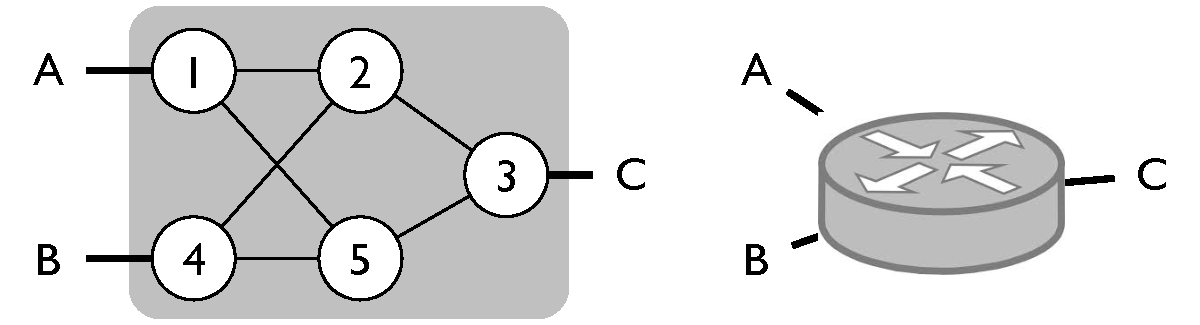
\includegraphics[width=.95\linewidth]{eg-one-big-switch.pdf}
  \caption{\footnotesize Example network and its one big switch
    abstraction}
  \label{fig:eg-one-big-switch}
\end{figure}
\vspace{-1em}

\Paragraph{As base tables} represent a network's
forwarding state, its role is to hide hardware heterogeneity, enable
transaction processing, and ease the creation of external
abstractions. Hence, they hold all the network
(configuration) data in a unified form that is easily accessible.  A
natural choice is a relational model~\cite{hull_relative_1984} that 
consists of three tables: \nd{topology} table that models network as a
pool of resource capacity, \nd{configuration} table that is the union
of all FIBs, and an optional \nd{constraint} table for 
network constraints (\eg SLAs).  \Eg Table~\ref{table:base-table}
shows example table instances.
% annotated topology table~\ref{tb:topology} represents the network's
% resource limit, whereas the flow table
% configuration~\ref{tb:configuration} is a snapshot of the network's
% allocated resource.
All tables are populated when the network is set up (assuming the FIBs
configured pro-actively), and incrementally updated afterwards as
network topology and/or configuration changes.

\begin{table}[ht!]
\begin{subtable}[t]{0.5\linewidth}
  {
    \footnotesize
    \subcaption{topology}
      \begin{tabular}[t!]{c|c|c|c}
        \centering
        node & node & avail\_bw  & used\_bw \\
        \hline
        1 & 2 & 3 & 2 \\
        1 & 5 & 5 & 0 \\
        \multicolumn{4}{c}{...}\\
        \hline
        4 & 5 & 5 & 0 \\
        4 & 2 & 5 & 0 \\ 
        \multicolumn{4}{c}{...}
        \label{tb:topology}
    \end{tabular}
  }
\end{subtable}
\;
\begin{subtable}[t]{0.45\linewidth}
  {
    \footnotesize
    \subcaption{per\_switch configuration}
    \centering
    \begin{tabular}[t]{c|c |c|c}
      \centering
      switch & flow & next & bw \\
      \hline
      1 & 1 & 2 & 1 \\
      1 & 2 & 2 & 1  \\
      \multicolumn{4}{c}{...}\\
      \hline
      2 & 1 & 3 & 1 \\
      \multicolumn{4}{c}{...}\\
      \hline
      3 & 1 & C & 1 \\
      \multicolumn{4}{c}{...}
      \label{tb:configuration}
    \end{tabular}
  }
\end{subtable}
\caption{\footnotesize Example base tables}
\label{table:base-table}
\end{table}
\vspace{-1em}

\Paragraph{The user-defined virtual views} are external
abstractions interfacing with users that are derived from the base tables as SQL
queries and serve as a logical perspective for a user's task. Compared to the
logical contexts introduced in earlier
works~\cite{ethane-sigcomm07,virtual-forwarding-plane}, the strength
of \Sys views is that it does not confine users to preselected
frozen abstractions, instead \Sys views can be created and changed by
users on demand by simply issuing or modifying a SQL query,
which selects from the distributed base tables the relevant
information and restructures them into a network-wide data-structure
that fits the user's task.

\begin{table}[ht!]
  \centering
\begin{subtable}[t]{0.3\linewidth}
    \centering
  {\footnotesize
    \subcaption{routing policy}
      \begin{tabular}[t]{c|c}
        flow & path\_vector \\
        \hline
        1 & (1,2,3) \\
        2 & (1,2,4) \\
        3 & (4,5,3) \\
        \multicolumn{2}{c}{...}
        \label{tb:routing} 
    \end{tabular}
    }
  \end{subtable}
  \;
  \begin{subtable}[t]{0.33\linewidth}
    \centering
  {\footnotesize
    \subcaption{end\_to\_end policy}
    \begin{tabular}[t]{c|c|c}
      flow & ingress & egress \\
      \hline
      1 & 1 & 3 \\
      2 & 1 & 4 \\
      3 & 4 & 3 \\
      \multicolumn{3}{c}{...}
      \label{tb:endpoint}
    \end{tabular}
    }
  \end{subtable}
  \;
  \begin{subtable}[t]{0.3\linewidth}
    \centering
  {\footnotesize
    \subcaption{one\_big\_switch}
    \begin{tabular}[t]{c|c}
        flow & next \\
        \hline
        1 &  C  \\
        2 & B \\
        3 & C \\
        \multicolumn{2}{c}{...}
        \label{tb:rule-capacity}
      \end{tabular}
    }
  \end{subtable}        
  \caption{\footnotesize Example views.}
\label{table:eg-views}
\end{table}

For example, a network-wide routing policy is nothing but the abstract
data as a view (Table~\ref{tb:routing}), derived from the per-switch
\nd{configuration} table, by the following query:
\begin{sql}
CREATE VIEW routing_policy AS (
  SELECT DISTINCT c.flow_id, fp.path_vector
  FROM configuration c 
       NATURAL JOIN flow_policy_fun(c.flow_id) fp
  ORDER BY c.flow_id );  
\end{sql}
In line 2, the \nd{select} statement selects two attributes to from
the view schema: attribute \nd{flow\_id} from \nd{configuration} and
\nd{path\_vector} from \nd{flow\_policy\_fun} which is a recursive
function that computes routing path for \nd{flow\_id}. 
% The \nd{JOIN} statement allows flows to be returned in the absence
% of configuration.  The resulting table of two attributes
% \nd{flow\_id} and \nd{path\_vector} forms the \nd{routing\_policy}
% view.
Similarly, we can derive a one-big-switch configuration view from
\nd{configuration} table and the \nd{obs\_mapping} table which keeps
tracks of the constituting physical nodes \nd{p\_node}.
\begin{sql}
CREATE VIEW obs_configuration AS (
  SELECT flow_id, t.next_id
  FROM   configuration t INNER JOIN obs_mapping ob
  ON     t.switch_id = ob.p_node );  
\end{sql}

Since a view is virtual, only its definition (the query) is stored.
Codd's relational model ensures that a SQL query outputs nothing but tables
(relations), allowing users to use views exactly as a table. A direct
usage is to create views on top of views. The next example shows how to
create an end-to-end policy (Table~\ref{tb:endpoint}) view from
\nd{routing\_policy} view:
\begin{sql}
CREATE VIEW e2e_policy AS (
 SELECT flow_id,
       path_vector[1] AS ingress,
       path_vector[array_length(path_vector,1)] AS egress
 FROM  routing_policy
 ORDER BY flow_id ) ;  
\end{sql}
 

\section{View Interface}
\label{sec:details}

The design goal of \Sys view interface is to combine the strength of
the following:
\begin{itemize}
\item An interface that loads and transforms the dataplane states.
  % structured in a format that eases control logic.
  The challenge is to
  identify a small set of views that are also expressive enough for
  common networking tasks. (\S~\ref{subsec:view-library})
\item Composition. (\S~\ref{subsec:compose})
\item Built-in services of real-time verification and
  synthesis. (\S~\ref{sec:veri-syn})
\item Performance. The challenge is that a naive implementation of
  relational queries does not scales well for the networking setting
  of SDN, where most interesting abstractions, by nature, will call
  for path-related computation that is recursive, and hence expensive
  in the naive implementation. (\S~\ref{sec:eval})
\end{itemize}

To achieve all the above, \Sys features a library of view primitives.
... create abstractions on the fly that can be categorized in two
groups: (1) the per-flow views ... We also call this type ``local
views'', because ... (2) the network-wide views ... we call this type
``global views''.  (1) enables real-time verification and synthesis;
(2) provides the interface for integrating network-wide service such
as traffic engineering.  This section presents (1,2) in
details. Services and performance are discussed in
\S~\ref{sec:veri-syn} and \S~\ref{sec:eval}.

\subsection{Abstraction hierarchy}

\label{subsec:view-library}

\subsection{Base tables}

Before introducing the derived views, let us first discuss in depth
the base tables -- the flat universe of networking data that are
actually stored in the database. The base tables serve two roles: (1)
a flat universe of tables to which all network configuration states
and state changes can be easily loaded; (2) the bases for building
layers of view abstractions where the reverse view update shall be
(relatively) easy.

\begin{sql}
CREATE OR REPLACE FUNCTION reachability_perflow(f integer)
RETURNS TABLE (flow_id int, source int, target int, hops bigint) AS 
$$
BEGIN
	DROP TABLE IF EXISTS tmpone;
	CREATE TABLE tmpone AS (
	SELECT * FROM configuration c WHERE c.flow_id = f
	) ;

	RETURN query 
        WITH ingress_egress AS (
		SELECT DISTINCT f1.switch_id as source, f2.next_id as target
       	      	FROM tmpone f1, tmpone f2
	      	WHERE f1.switch_id != f2.next_id AND
		      f1.switch_id NOT IN (SELECT DISTINCT next_id FROM tmpone) AND
	              f2.next_id NOT IN (SELECT DISTINCT switch_id FROM tmpone)
                ORDER by source, target),
	     reach_can AS(
                SELECT i.source, i.target,
	      	       (SELECT count(*)
                        FROM pgr_dijkstra('SELECT 1 as id,
			     	           switch_id as source,
					   next_id as target,
					   1.0::float8 as cost FROM tmpone',
			     i.source, i.target,TRUE, FALSE)) as hops
	        FROM ingress_egress i)
	SELECT f as flow_id, r.source, r.target, r.hops FROM reach_can r where r.hops != 0;
END
$$ LANGUAGE plpgsql;
\end{sql}

\subsection{Virtual views}

\subsubsection{View primitives}

\Paragraph{Per-flow forwarding graph and reachability views}

Lies in the heart of any pair-wise reachability views, be it
reachability for a plain network, for an one-big-switch network, or
for an arbitrary virtual network, is a query like the following:
 
% \begin{sql}
% SELECT source, 
%        target,
%        (SELECT count(*)
%         FROM pgr_dijkstra('SELECT * FROM """ + fg_view_name + """',
%              source, target, TRUE, FALSE)) AS hops
% FROM ingress_egress_pairs
% \end{sql}

% \begin{sql}
% def generate_forwarding_graph (cursor, flow_id):

%     fg_view_name = "fg_" + str (flow_id)

%     try:
%         cursor.execute("""
%         CREATE OR REPLACE view """ + fg_view_name + """ AS (
%         SELECT 1 as id,
%                switch_id as source,
% 	       next_id as target,
% 	       1.0::float8 as cost
%         FROM configuration
%         WHERE flow_id = \%s
%         );
%         """, ([flow_id]))

%     except psycopg2.DatabaseError, e:
%         print "Unable to create fg_view table for flow " + str (flow_id)
%         print 'Error \%s' \% e    
% \end{sql}

% \begin{sql}
% def generate_reachability_perflow (cursor, flow_id):

%     fg_view_name = "fg_" + str (flow_id)
%     reach_view_name = "reachability_" + str (flow_id)

%     try:
%         cursor.execute("""
%         CREATE OR REPLACE view """ + reach_view_name + """ AS (
%           WITH ingress_egress AS (
%                SELECT DISTINCT f1.source, f2.target
%                FROM """ + fg_view_name + """ f1, """ + fg_view_name + """ f2
%                WHERE f1.source != f2.target AND
%                      f1.source NOT IN (SELECT DISTINCT target FROM """ + fg_view_name +""") AND
%                      f2.target NOT IN (SELECT DISTINCT source FROM """ + fg_view_name +""" )
%                ORDER by f1.source, f2.target),
%                ingress_egress_reachability AS (
%                SELECT source, target,
%                       (SELECT count(*)
%                        FROM pgr_dijkstra('SELECT * FROM """ + fg_view_name + """',
%                                          source, target, TRUE, FALSE)) AS hops
%                FROM ingress_egress)
%           SELECT * FROM ingress_egress_reachability WHERE hops != 0
%         );""")

%     except psycopg2.DatabaseError, e:
%         print "Unable to create reachability table for flow " + str (flow_id)
%         print 'Error \%s' \% e      
% \end{sql}

% This section presents a prototype design of \TI in more details,
% showing preliminary evaluation with promising results.

% \Paragraph{Update views}



\subsubsection{View composition}
\label{subsec:compose}

From user perspective, a network view is a derived table that offers
the same tabular interface as ordinary (\ie materialized table that is
actually stored) tables. This allows to a stacking of views ...  ...
We use ``composition'' to loosely refer to the derivation of views
from existing views. ...

Consider one big switch, its per-flow forwarding graph view can be
built on top of per-flow forwarding graph view and one big switch
topology view, as follows:
\begin{sql}
CREATE OR REPLACE VIEW obs_1_fg_36093_3 AS (
       select 1 as id,
       	      switch_id as source,
	      next_id as target,
	      1.0::float8 as cost
       FROM obs_1_topo, fg_36093
       WHERE switch_id = source AND next_id = target
       ORDER BY source, target
);
\end{sql}

Note that, \nd{fg\_36093} is used as a filter for selecting
\nd{obs\_1\_topo} records that ... Symmetrically, one could also
``reverse'' the filtering and use \nd{fg\_36093} as a filter instead,
as follows:
\begin{sql}
CREATE OR REPLACE VIEW obs_1_fg_36093_4 AS (
       select 1 as id, source, target, 
	      1.0::float8 as cost
       FROM obs_1_topo, fg_36093
       WHERE switch_id = source AND next_id = target
       ORDER BY source, target
);
\end{sql}


While the above two view composition, namely SQL join, is very
intuitive: its body of ``view join'' directly translates. It is no
longer updatable. ... As an alternative equivalent view is by
... where one table is used as an ... parameter ...
\begin{sql}
CREATE OR REPLACE VIEW obs_1_fg_36093_2 AS (
       select 1 as id,
       	      switch_id as source,
	      next_id as target,
	      1.0::float8 as cost
       FROM configuration NATURAL JOIN topology
       WHERE flow_id = 36093 AND subnet_id = 1
       ORDER BY source, target
);
\end{sql}

To make advantage of view updates, \Sys adopts this
approach. Unfortunately, views are not allowed to be paramterized in
SQL standard. To achieve the affect of parameterized views, \Sys uses
Python wrapper as walk-round, as follows:



\section{Verification and synthesis}
\label{sec:veri-syn}

This section presents in more details the view interface and their
usage by three examples, namely real-time verification and synthesis
that are fully automatically enabled by database for virtual network,
one big switch, and distributed firewalls.

% three example view abstractions, together with the fully automatic
% verification and synthesis services,

\Subsection{Verification and synthesis as data synchronization}

% \todo{(this subsection) HotNet texts, will rework}

A network is in constant change. A virtual view is useful only if its
records are fresh -- reflecting the latest network instantly. For
example, when per-switch rules change, a query on the high-level
policy view \nd{e2e\_routing} (Table~\ref{tb:endpoint}) shall
automatically returns the updated \nd{e2e} reachability. Conversely,
to enable network manipulation via views, the base tables need to be
updated to reflect operations on the views.  For example, to set a new
route \nd{(1,5,4)} for \nd{flow 1} in the example network
(Figure~\ref{fig:eg-one-big-switch} (left)), a user simply insert a new
record denoting the path into the \nd{routing\_policy} view with
\nd{flow} attribute set to \nd{1}. \Sys is responsible of pushing this
abstract view insert into the relevant base \nd{configuration}
inserts.

Generally, view maintenance that keeps virtual views fresh and view
update that synthesizes the base table changes, jointly form a
bi-directional data synchronizer between the base and the view. While
modern DBSes implement view maintenance very efficiently, view update
is supported for restricted
cases~\cite{ak-view-udpate-thesis,relational-lenses}. This is no
surprise, as view update is the harder one: a view contains only partial
information of the base, it is not always possible to locate a unique
base table update~\cite{Bancilhon:view-update-semantics}. To enable
network operations on views, \Sys takes advantage of existing view
maintenance implementation and extends the support of view updates to
network view updates.

\Paragraph{Real-time view maintenance enables network verification.}
\textit{View maintenance} is well supported in modern database systems
(DBS), which \Sys adopts straightforwardly. Specifically, when a view
generated by SQL query program $q$, is queried by a SQL program $p$,
view maintenance translates $p$ on $q$ into queries $p \circ q$ on the
base tables.
% , hence always returning information that is update to the latest
% network state. On the other hand, since views are virtual, This very
% fast re-computation of $p$ keeps the view fresh.  requiring
% re-computation every time it is referred, an alternative is to
% materialize (actually store) the view to accelerate query on the
% views. In this case, view maintenance incrementally updates the
% materialized view table with regard to base table change.
Interestingly, view maintenance offers exactly what is needed in
real-time network verification: by specifying the property of interests
as $p$ over $q$, view maintenance performs check of $p \circ q$ on
network states on the fly. % As shown in \S~\ref{sec:eval},
% checking reachability on a network with more than 10k nodes costs
% less than 10 ms, magnitudes smaller compared to the typically
% per-rule installation or TE operation delay~\cite{b4,ffc}.

\Paragraph{Real-time view update enables network synthesis.}  
Given the ambiguity and non-existence in view update, we first
characterize the correctness criteria in networking. We identify
updates that keep a view's independent and complementary counter-parts
constant. Two views are \textit{independent} if the update on one does
not affect that on the other. Two views are \textit{complementary}, if
they contain enough information to recover the base tables.
% , \ie there alawys exists some base table updates that correctly
% reflect the updated view while keeping the rest views constant.
% In \Sys, it is desirable for views to be independent so they don't
% conflict each other. 
A view updates that keeps the independent views constant eliminates
accident changes made to other existing views; An update that keep a
view's \textit{complementary} constant is a stronger requirement that
does not pollute any possible views (existing and future ones).

\Sys assumes user views are independent, and only performs updates
that keep independent views constant.  In the current prototype, view
update is implemented by hand coded triggers, the call-back functions
that are automatically fired to update the bases when the associated
view update is issued. We evaluate this manual implementation (details
in \S~\ref{sec:eval}) to measure the DB induced delay.
Ultimately, \Sys aims for a generic view update algorithm that
synthesizes for any user-defined views. (We have sketched a novel
algorithm, omitted due to space.) We leave the implementation of the
generic algorithm for future work.

% \input{preliminary-eval}


% \subsection{Verification example}

% \subsection{Synthesis example}

\subsection{Virtual network}

\begin{sql}
select * from vn_reachability where flow_id = 77899 ;
 flow_id | ingress | egress 
---------+---------+--------
   77899 |     486 |     19  
   ...
\end{sql}

This entry corresponds to a record in configuration as follows:
\begin{sql}
SELECT flow_id, pv FROM configuration_pv WHERE flow_id = 77899;
---------+----------------------------------
 flow_id |                pv                
   77899 | {486,498,462,463,456,472,109,19}
\end{sql}

To update the virtual network policy that revoke transient service for
flow \nd{77899} between ingress \nd{486} and egress \nd{19}, the user
could direcly modify the \nd{vn\_reachability} table by deleting the
corresponding record as follows:
\begin{sql}
DELETE FROM vn_reachability WHERE 
        flow_id = 27079 AND ingress = 486 AND egress = 19;  
\end{sql}

This deletion results in the deletion of three switch-level
configurations as follows:
\begin{sql}
[[462, 463], [486, 498], [498, 462]]  
\end{sql}
The reason that only three entries at switches \nd{462, 486, 498} are
removed is that the rest of the ... are 

\begin{sql}
SELECT flow_id, pv FROM configuration_pv WHERE flow_id = 77899;
 flow_id |                pv                
---------+----------------------------------
   77899 | {483,463,456,472,109,19}
   77899 | {486,498,462,463,456,472,109,19}
   ...
\end{sql}

Similarly, on user request for adding new or updating exiting virtual
network end to end policy, \Sys synthesizes the relevant switch-level
configuration modification.
Add new policy:
\begin{sql}
INSERT INTO vn_reachability VALUES (55716, 557, 483);  
\end{sql}

Update policy:
\begin{sql}
UPDATE vn_reachability SET egress = 230
        WHERE flow_id = 97940 AND ingress = 497;  
\end{sql}

Finally, it is worth noting that, a policy update request may not
always be valid. For example, a deletion of policy \nd{(42692, 497,
  375)} in ... 

\begin{sql}
SELECT source, target, pv FROM configuration_pv WHERE flow_id = 42692;
 source | target |                pv                 
--------+--------+-----------------------------------
    486 |    375 | {486,498,462,463,456,472,108,375}
    497 |    230 | {497,462,463,456,230}
    497 |    375 | {497,462,463,456,472,108,375}
    ...
\end{sql}

While \Sys, which utilizes the default view updates mechanism
implemented by postgres, will simply remove policy \nd{(42692, 497,
  375)} from \nd{vn\_reachability} view, and leaves the per-switch
configuration unchanged. 
% \begin{sql}
% Switch delta after del of 42692 between 497 and 375 []
% \end{sql}

\subsection{One big switch abstraction}

\subsection{Distributed firewall}

\begin{sql}
ALTER VIEW reachability_rel_obs_out2 ALTER COLUMN source SET DEFAULT 591;  
\end{sql}

 
% \section{Realtime synthesis}



\section{Evaluation}
\label{sec:eval}


We develop a prototype featuring view interface and
verification/synthesis services. Our prototype serves two purposes:
First, we use it to study the feasibility of managing SDN data-plane
with database. In particular, we gathered performance overhead
introduced by database on various ISP topologies (up to ) with
configurations initialized with real routeview feeds (2
million). ... ; Second, with the prototype, we explored two
fundamental tradeoff: expressiveness (of views) versus operation
performance, and automation (of updates) versus performance. We
conclude that ...

The prototype is implemented in PostgreSQL~\cite{postgres}, an
advanced database that is popular for both academia and commercial
use, on ... % on a laptop with 1.80GHz Intel Core i7-4500U CPU and 2GB RAM,
% running Ubuntu 14.04 LTS.

\subsection{Scalability}

\begin{figure}
  \centering
  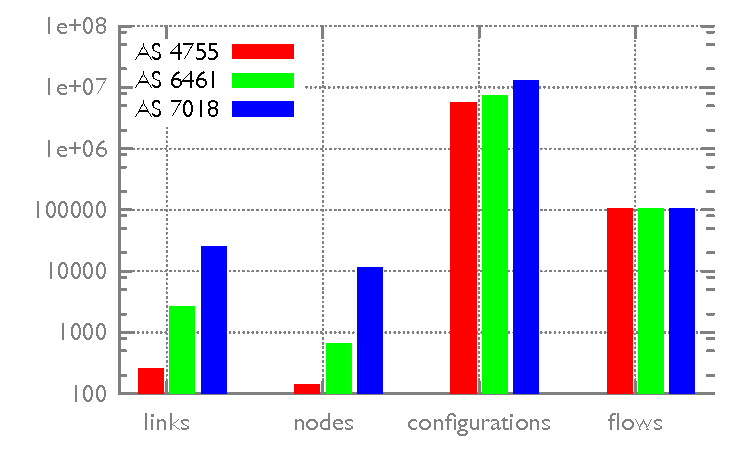
\includegraphics[width=1\linewidth]{figures/init.pdf}
  \caption{Configuration size.}
  \label{fig:init}
\end{figure}

\begin{figure}
  \centering
  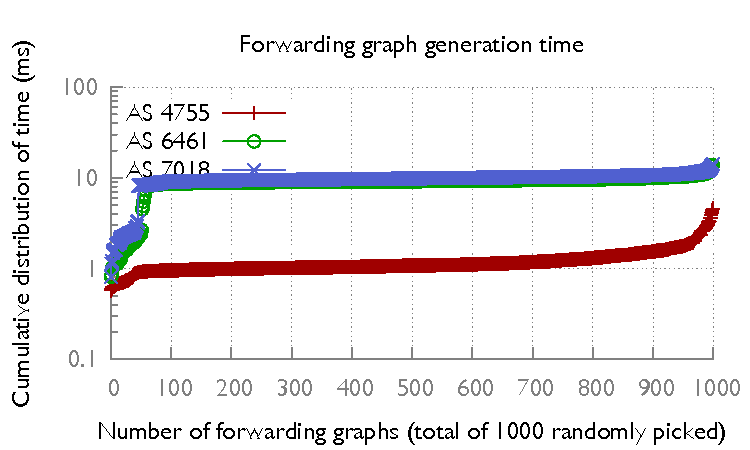
\includegraphics[width=1\linewidth]{figures/fg_cdf1000.pdf}
  \caption{Forwarding graph generation.}
  \label{fig:init}
\end{figure}

\begin{figure}
  \centering
  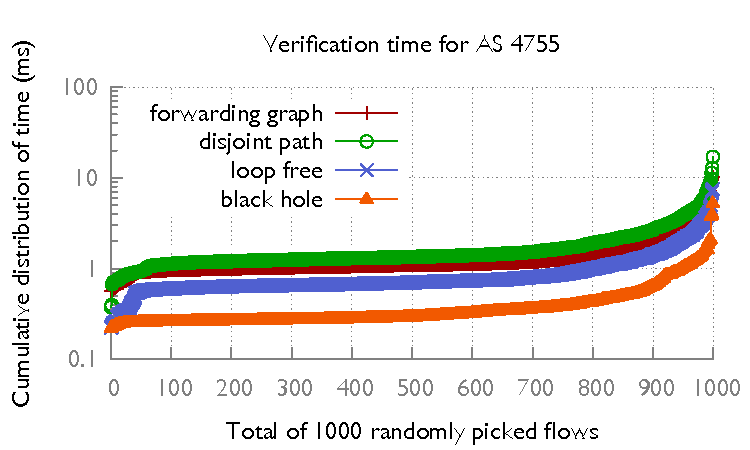
\includegraphics[width=1\linewidth]{figures/verify_cdf1000.pdf}
  \caption{Verification Time.}
  \label{fig:init}
\end{figure}

\begin{figure}
  \centering
  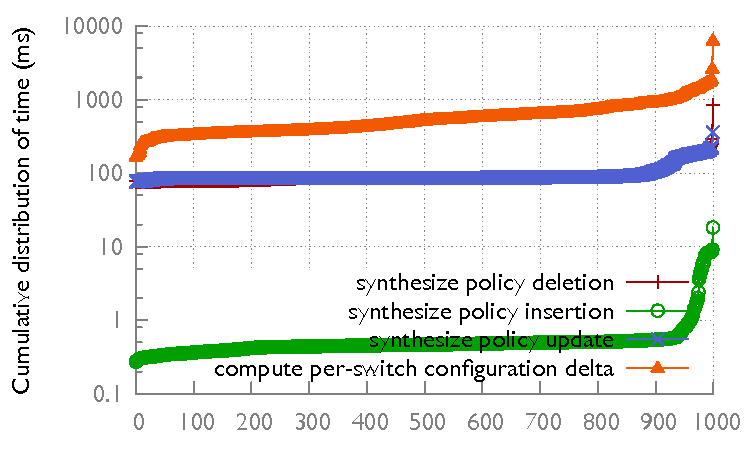
\includegraphics[width=1\linewidth]{figures/vn_synthesis_cdf1000.pdf}
  \caption{Synthesis Time.}
  \label{fig:init}
\end{figure}

\subsection{Tradeoff: expressivenss, automation, and performance}

% \begin{figure*}
%   \centering
%   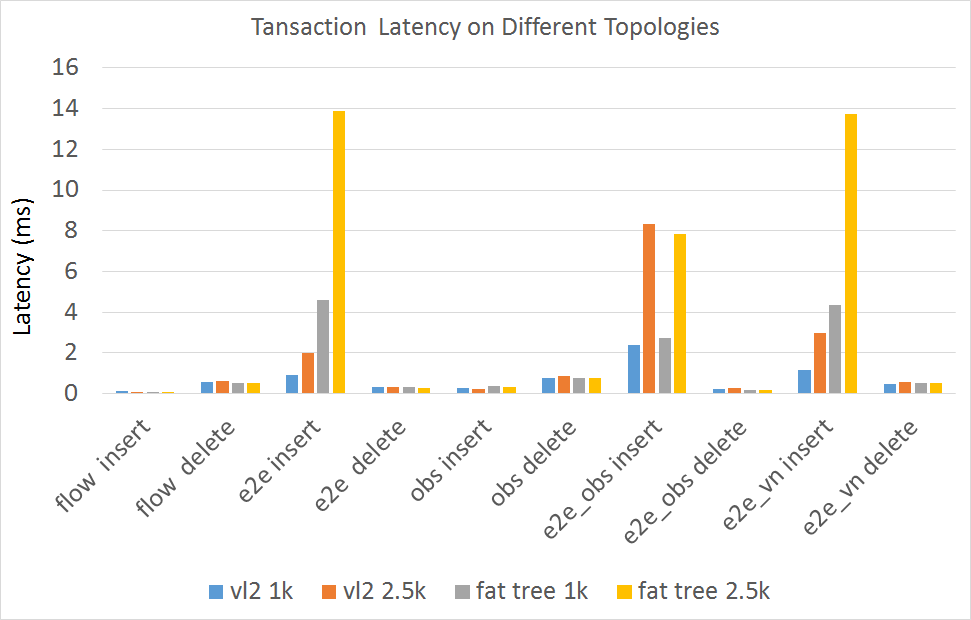
\includegraphics[width=1\linewidth]{transaction_latency.png}
%   \caption{Latency of transactions against different topologies.}
%   \label{fig:latency-all}
% \end{figure*}

% % GNUPLOT: LaTeX picture
\setlength{\unitlength}{0.240900pt}
\ifx\plotpoint\undefined\newsavebox{\plotpoint}\fi
\sbox{\plotpoint}{\rule[-0.200pt]{0.400pt}{0.400pt}}%
\begin{picture}(1500,900)(0,0)
\sbox{\plotpoint}{\rule[-0.200pt]{0.400pt}{0.400pt}}%
\put(151.0,146.0){\rule[-0.200pt]{4.818pt}{0.400pt}}
\put(131,146){\makebox(0,0)[r]{ 6}}
\put(1419.0,146.0){\rule[-0.200pt]{4.818pt}{0.400pt}}
\put(151.0,221.0){\rule[-0.200pt]{4.818pt}{0.400pt}}
\put(131,221){\makebox(0,0)[r]{ 7}}
\put(1419.0,221.0){\rule[-0.200pt]{4.818pt}{0.400pt}}
\put(151.0,296.0){\rule[-0.200pt]{4.818pt}{0.400pt}}
\put(131,296){\makebox(0,0)[r]{ 8}}
\put(1419.0,296.0){\rule[-0.200pt]{4.818pt}{0.400pt}}
\put(151.0,372.0){\rule[-0.200pt]{4.818pt}{0.400pt}}
\put(131,372){\makebox(0,0)[r]{ 9}}
\put(1419.0,372.0){\rule[-0.200pt]{4.818pt}{0.400pt}}
\put(151.0,447.0){\rule[-0.200pt]{4.818pt}{0.400pt}}
\put(131,447){\makebox(0,0)[r]{ 10}}
\put(1419.0,447.0){\rule[-0.200pt]{4.818pt}{0.400pt}}
\put(151.0,522.0){\rule[-0.200pt]{4.818pt}{0.400pt}}
\put(131,522){\makebox(0,0)[r]{ 11}}
\put(1419.0,522.0){\rule[-0.200pt]{4.818pt}{0.400pt}}
\put(151.0,598.0){\rule[-0.200pt]{4.818pt}{0.400pt}}
\put(131,598){\makebox(0,0)[r]{ 12}}
\put(1419.0,598.0){\rule[-0.200pt]{4.818pt}{0.400pt}}
\put(151.0,673.0){\rule[-0.200pt]{4.818pt}{0.400pt}}
\put(131,673){\makebox(0,0)[r]{ 13}}
\put(1419.0,673.0){\rule[-0.200pt]{4.818pt}{0.400pt}}
\put(151.0,748.0){\rule[-0.200pt]{4.818pt}{0.400pt}}
\put(131,748){\makebox(0,0)[r]{ 14}}
\put(1419.0,748.0){\rule[-0.200pt]{4.818pt}{0.400pt}}
\put(321.0,131.0){\rule[-0.200pt]{0.400pt}{4.818pt}}
\put(321,90){\makebox(0,0){ 1.2}}
\put(321.0,756.0){\rule[-0.200pt]{0.400pt}{4.818pt}}
\put(549.0,131.0){\rule[-0.200pt]{0.400pt}{4.818pt}}
\put(549,90){\makebox(0,0){ 1.4}}
\put(549.0,756.0){\rule[-0.200pt]{0.400pt}{4.818pt}}
\put(777.0,131.0){\rule[-0.200pt]{0.400pt}{4.818pt}}
\put(777,90){\makebox(0,0){ 1.6}}
\put(777.0,756.0){\rule[-0.200pt]{0.400pt}{4.818pt}}
\put(1004.0,131.0){\rule[-0.200pt]{0.400pt}{4.818pt}}
\put(1004,90){\makebox(0,0){ 1.8}}
\put(1004.0,756.0){\rule[-0.200pt]{0.400pt}{4.818pt}}
\put(1232.0,131.0){\rule[-0.200pt]{0.400pt}{4.818pt}}
\put(1232,90){\makebox(0,0){ 2}}
\put(1232.0,756.0){\rule[-0.200pt]{0.400pt}{4.818pt}}
\put(151.0,131.0){\rule[-0.200pt]{0.400pt}{155.380pt}}
\put(151.0,131.0){\rule[-0.200pt]{310.279pt}{0.400pt}}
\put(1439.0,131.0){\rule[-0.200pt]{0.400pt}{155.380pt}}
\put(151.0,776.0){\rule[-0.200pt]{310.279pt}{0.400pt}}
\put(30,453){\makebox(0,0){Counts}}
\put(795,29){\makebox(0,0){Times (ms)}}
\put(795,838){\makebox(0,0){Gnuplot Example}}
% \put(1279,736){\makebox(0,0)[r]{'exp.dat' u 1:2:(sqrt($2))}}
\put(1299.0,736.0){\rule[-0.200pt]{24.090pt}{0.400pt}}
\put(1299.0,726.0){\rule[-0.200pt]{0.400pt}{4.818pt}}
\put(1349,736){\makebox(0,0){$+$}}
\put(1399.0,726.0){\rule[-0.200pt]{0.400pt}{4.818pt}}
\put(151.0,131.0){\rule[-0.200pt]{0.400pt}{155.380pt}}
\put(151.0,131.0){\rule[-0.200pt]{310.279pt}{0.400pt}}
\put(1439.0,131.0){\rule[-0.200pt]{0.400pt}{155.380pt}}
\put(151.0,776.0){\rule[-0.200pt]{310.279pt}{0.400pt}}
\end{picture}


% \begin{figure*}[ht!]
%         \centering
%         \begin{subfigure}[b]{.4\linewidth}
%           \centering
%           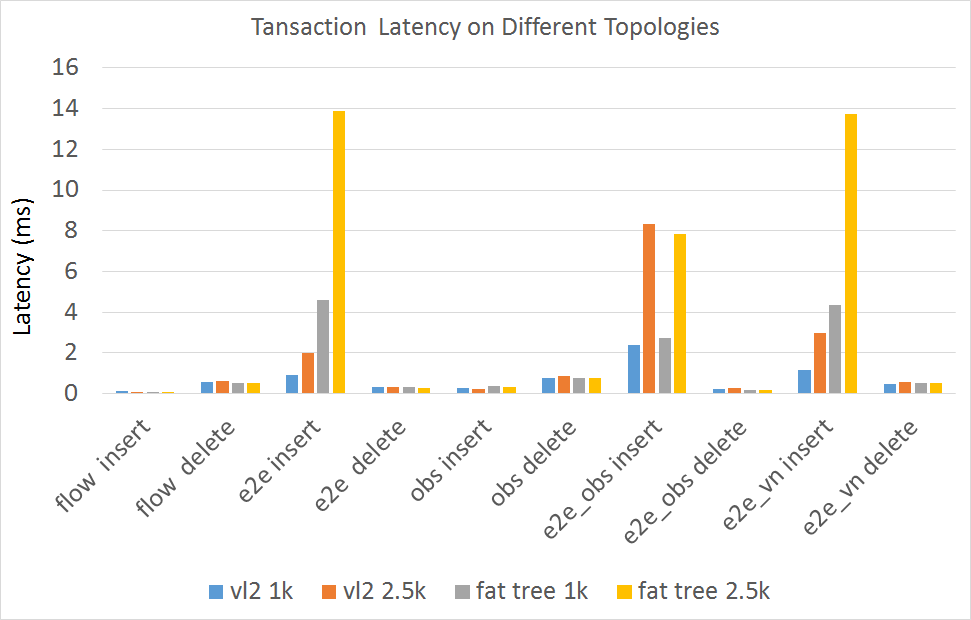
\includegraphics[width=1\textwidth]{transaction_latency.png}
%   \caption{Latency of transactions against different topologies.}
%   \label{fig:latency-all}
%           % \includegraphics[width=1\textwidth]{fig-SDNandDB-cropped.pdf}
%           % \caption{\textit{\textbf{SDN architecture (left)}},
%           %   \textit{\textbf{database architecture
%           %       (right)}}. \textit{\textbf{SDN networks}} offers a
%           %   centralized logical view of the network infrastructure:
%           %   app/users see the same complex network states, controller
%           %   carefully handles name/device binding;
%           %   \textit{\textbf{database}} bridges user and data by two
%           %   separate data abstractions: logical base tables hide
%           %   physical heterogeneity, external views interface end
%           %   users, \textbf{view maintenance and update} synchronize
%           %   the two.}
%           % \label{fig:SDNandDB}
%         \end{subfigure}
%         \hfill
%         \begin{subfigure}[b]{.232\linewidth}
%   \centering
%   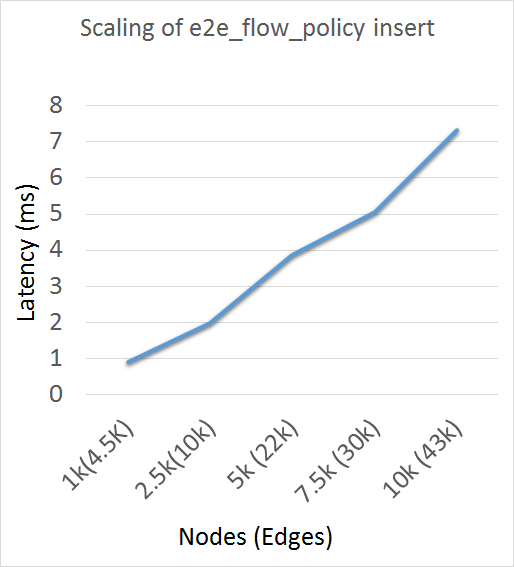
\includegraphics[width=1\textwidth]{scaling.png}
%   \caption{Latency against network size.}
%   \label{fig:trend}
%         \end{subfigure}
%         \begin{subfigure}[b]{.35\linewidth}
% \begin{center}
%     \small 
% \begin{tabular}{ | l | c | c |}
% \hline
% \textbf{operation} & \textbf{st (10ms)} & \textbf{ st (1s) }  \\
% \hline
% \hline
% flow insert  	 & 	91	&	9,091 \\
% \hline
% flow delete 	&	17	&	1,695 \\
% \hline
% e2e insert	& 16	&	1,563 \\
% \hline
% e2e delete   &  32	&	3,226 \\
% \hline
% obs insert	      & 	29	&	2,857 \\
% \hline
% obs  delete	&  16	&	1,587 \\
% \hline
% e2e\_obs insert	&  	15	&	1,471 \\
% \hline
% e2e\_obs delete & 	37	&	3,704 \\
% \hline
% e2e\_vn insert	&	23	&	2,273 \\
% \hline
% e2e\_vn delete	&	21	&	2,128 \\
% \hline
% \end{tabular}
% \end{center}
% 	\caption{STF measure for 100-node VL2 with 404 edges.\label{fig:stf}}
%   % \centering
%   % 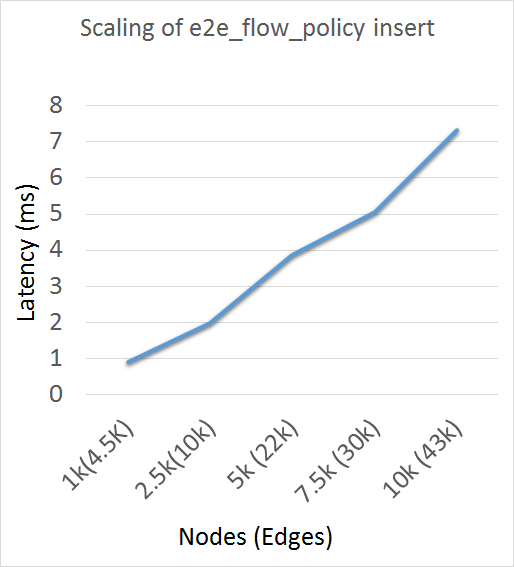
\includegraphics[width=1\textwidth]{scaling.png}
%   % \caption{Scaling of latency with network size.}
%   % \label{fig:trend}
%         \end{subfigure}
%         \caption{\footnotesize \Sys induced latency very small compared to the
%           switching rule update time}\label{fig:eval}
% \end{figure*}
% % \vspace{-3em}

% A prototype of several core features \TI demonstrates promising
% performance, showing that \Sys induced per-rule latency is less than
% 14 ms for all network instances up to 10k nodes, achieving very high
% STF (switch-time fraction) and linear growth as network size
% increases. 

% Specifically, Figure~\ref{fig:latency-all} summarizes the latency (in
% millisecond) induced by DB operation for each FIB update.  For each
% table in the x-axis: base table \nd{flow} (per-switch rule), view
% \nd{e2e} (end to end policy on physical network), \nd{obs}
% (one-big-switch configuration), \nd{obs\_e2e} (e2e policy for
% one-big-switch), and \nd{e2e\_vn} (e2e policy for virtual network), we
% run two operation, insert of a new record, and deletion of an existing
% one, where delay is computed on four networks, \nd{vl2 1k, 2.5k} (VL2
% topology with 1k and 2.5k nodes), and \nd{fat\_tree 1k, 2.5k}. The
% delay for all instances is on the scale of 1-14 ms. We also observe
% that inserts incur most noticeable delay for
% \nd{e2e,e2e\_obs,e2e\_vn}, since the \nd{e2e} view insert involves an
% extra step of path selection between the end nodes. In addition,
% Figure~\ref{fig:trend} shows the linear growth of \Sys induced latency
% as network size increases from 1k to 10k on VL2 topology.  And
% Figure~\ref{fig:stf} computes for each DB operation the switch time
% fraction (STF = $\frac{Switch\;\; time}{DB\; induced\; delay\; time}$)
% on 100-node VL2 network with switch time of 10ms (the average rule
% update time on a controlled network of 100 nodes~\cite{ffc}) and 1 sec
% (a representative time in B4 network~\cite{b4}).

% \begin{figure}[h]
% \begin{center}
%     \footnotesize
% \begin{tabular}{ | l | c | c |}
% \hline
% operation & st(10ms) & st(1s)  \\
% \hline
% \hline
% flow insert  	 & 	91	&	9,091 \\
% \hline
% flow delete 	&	17	&	1,695 \\
% \hline
% e2e insert	& 16	&	1,563 \\
% \hline
% e2e delete   &  32	&	3,226 \\
% \hline
% obs insert	      & 	29	&	2,857 \\
% \hline
% obs  delete	&  16	&	1,587 \\
% \hline
% e2e\_obs insert	&  	15	&	1,471 \\
% \hline
% e2e\_obs delete & 	37	&	3,704 \\
% \hline
% e2e\_vn insert	&	23	&	2,273 \\
% \hline
% e2e\_vn delete	&	21	&	2,128 \\
% \hline
% \end{tabular}
% \end{center}
% 	\caption{STF measure for 100-node vl2 with 404 edges.\label{fig:stf}}
% \end{figure}



\section{Discussion and Future Work}
\label{sec:discussion}

\subsection{Network orchestration and view updates}

Discuss the semantics of view updates: An ideal case of view update
keeps a view's complement constant ... that is, a view update does not
impose side affects that may corrupt other views.

View updates ... briefly introduce existing works, connection to
recent provenance work.

\Paragraph{Real-time view update enables network synthesis.}  
Given the ambiguity and non-existence in view update, we first
characterize the correctness criteria in networking. We identify
updates that keep a view's independent and complementary counter-parts
constant. Two views are \textit{independent} if the update on one does
not affect that on the other. Two views are \textit{complementary}, if
they contain enough information to recover the base tables.
% , \ie there alawys exists some base table updates that correctly
% reflect the updated view while keeping the rest views constant.
% In \Sys, it is desirable for views to be independent so they don't
% conflict each other. 
A view update that keeps the independent views constant eliminates
accident changes made to other existing views; An update that keep a
view's \textit{complementary} constant is a stronger requirement that
does not pollute any possible views (existing and future ones).

\Sys assumes user views are independent, and only performs updates
that keep independent views constant.  In the current prototype, view
update is implemented by hand coded triggers, the call-back functions
that are automatically fired to update the bases when the associated
view update is issued. We evaluate this manual implementation (details
in \S~\ref{sec:eval}) to measure the DB induced delay.
Ultimately, \Sys aims for a generic view update algorithm that
synthesizes for any user-defined views. (We have sketched a novel
algorithm, omitted due to space.) We leave the implementation of the
generic algorithm for future work.

% \Paragraph{Forwarding plane updates via query optimization}
% \Paragraph{Network synthesis via database provenance}

\subsection{Consistent forwarding plane and transaction processing}

\todo{need re-write: but all raw texts are here}

Next, \Sys's \TR provides sequential and recoverable behavior of
concurrent user operations, with \textit{ACID} semantics:
sequentiality ensures user operations proceed \textit{atomically} and
are \textit{isolated} from one another, always leaving the network in
a \textit{consistent} state; and recoverability assures operation
failure does not pollute network state, leaving effects of committed
operation \textit{durable}. Unlike conventional database systems
(DBSes) where the operations, transaction, and their connections are
obvious~\cite{Bernstein:concurrency-recovery,concurrency-recovery-alg,principles-tp,concurrency-ddb},
the interpretation in networking is obscure, as observed in early
works~\cite{hotsdn-transactional-networking,On-Consistent-Updates,of-cpp}.
The inherent dilemma is that transaction, the logical unit that
preserves ACID, usually is meaningful only for network-wide actions;
whereas the enabling mechanism usually is only efficiently enforceable
for switch-level operation. \TTR solves this by leveraging the view
abstraction introduced in \TI: transactions, like other high-level
operations, are specified over views; whereas the enforcing mechanisms
are built on base tables.  For example, if a transaction over a
particular view is processed via two-phase locking, according to that
view (the SQL query), \Sys translates locks over the abstract view
into a set of locks that can be performed locally at the relevant
distributed base tables.


Transactional networking offers an efficient execution abstraction of
user programs in a shared distributed network, freeing the user from
the challenging concurrency and recovery control
problem~\cite{consistency-lock,concurrency-recovery-alg,principles-tp,concurrency-ddb,Tc-ddb,crdb}.

\Paragraph{Transaction preserves ACID properties.} In \Sys, a
transaction is a logical unit of operations that are atomically and
isolated from one another, preserving network consistency and
preventing failure from polluting effects of already committed
transaction. The operations in a transaction are partially-ordered,
defined in the user program. An operation is either a read or write: a
write maps to network (re)configuration in the form of an insert or
delete\footnote{An update is a deletion followed by an insertion} of
records in a base table or view; a read, on the other hand, maps to
packet processing, since packet processing is the effect of ``read''
policy data. An example transaction is the collection of flow events
interleaved with network re-configurations issued by a user
program. By DB concurrency and recovery control, \Sys executes
transactions concurrency while retaining the ACID semantics.

\Paragraph{Transactions on views.}  
Like users interact with \Sys via views, they also conceive
transactions on views. Specifically, we write $(T,v, \overline{op})$
for a transaction $T$ with operation set $\overline{op}=op_1,\cdots
op_n$ on a view $v$.  Users tell \Sys of $T$ by wrapping his program
like the following:
\begin{sql}
Start; program (op1;...opn;) Commit;
\end{sql}
The key to efficient transaction processing for parallel programs is a
scheduler that coordinates data access of operations while preserving
ACID. It has been shown that the scheduling problem decompose to two
sub-problems: resolving conflicting read-write operations, and that
for write-write operations~\cite{Bernstein:concurrency-recovery}.
Read-write conflict occurs between a configuration update (write) and
processing of in-fly traffic (read) that will be affected by the
update; write-write conflict occurs when the updated data items
overlap. A standard scheduler that prevents both conflicts is
two-phase locking~\cite{Bernstein:concurrency-recovery} where a
transaction $(T,v,\overline{op})$ becomes $(T,v, (lock(v),
\overline{op}, unlock(v)))$, that is:
\begin{sql}
Start; lock(v); program (op1;...opn;) unlock(v); Commit;
\end{sql}

\Paragraph{Transactions on base tables at switches.} Transactions on
views are inefficient: a view is by nature application-specific,
typically network-wide, involving multiple distributed nodes (\eg that
forms a path).  Transactions over views require synchronization among
the participant nodes, making \nd{lock(v)} and \nd{unlock(v)} complex
tasks that lack performance.  Hence rather than adding concurrency and
recovery enforcement to views, \Sys implemented them at base tables,
where the locks can be performed locally at individual node.  To
enable this, \Sys translates a transaction $(T,v_{routing},
(lock(v_{routing}),op,unlock(v_{routing})))$ on a path defined by a
routing policy view $v_{routing}$ to a set of base table transactions
$(T,b_i, (lock_{b_i}, op_{b_i}, unlock_{b_i})) $ where $b_i$, the base
table derived from the view
($v_{routing}$). 
Operations on $b_i$ proceed independent of each other. When multiple
$T_i$ is executed, two-phase locking over views is achieved by
switch-level locking that enforce a consensus of partial ordering
among conflicting operations.

% \Paragraph{Relational vs. non-relational database} ...  Map-reduce
% ...  Networking services, unlike the ad-hoc lightweight ... However,
% relational database is a general purpose tool not designed for
% highly-connected data. That is, despite decades of relational
% database query optimization and indexing research, which brought its
% commerical success, those non-relational, graph database for
% example, outperforms relational database on query involving graph
% operations.


% \Paragraph{Non-relational database} ... semi-structured, graph
% database, ... 


% \section{Challenges}

\Paragrph{Data plane is a distributed system where datas are
  partitioned and replicated.}  The network-wide forwarding states are
partitioned across nodes

\Paragrph{Data plane is a distributed system with realtime demands}

% \Paragrph{Write operation (packet processing) in a unreliable data}

 

\vspace{-.5em}
\Section{Related work}
\label{sec:related}

\Paragraph{Network verification and synthesis}, despite recent
efforts~\cite{veriflow,NetPlumber,network-verification-in-light-of-pv,dnv},
have not matured into a wanted industry of standard reusable tools
with a general-purpose interface.  General-purpose verification tools,
despite powerful tools like SMT solvers, are not directly applicable
to network size; Domain-specific heuristics are fast but require extra
effort and are not reusable.  Formal synthesis is even harder and
slower: existing tools does not scale
well~\cite{reactive-synthesis-sdn}. By utilizing DB's general query
engine that has been optimized for two decades as the main reasoning
engine, \Sys brings new hope to a networking verifier that strikes a
balance between general-purpose support and realtime performance.  We
would throughly study the power and limits of \Sys's support for
realtime verification and synthesis.

\Paragraph{Views, authorization, and locking} are three inherently
connected concepts in database~\cite{Views-Authorization-and-Locking}:
views expose data, authorization prescribes access to data, and
locking implements authorization. Thus, the view-centric \Sys lends
itself to a rich body of locking based authorization mechanism that is
particularly straightforward and flexible: one may associate lock with
different operations \eg write or/and read, and data of different
granularity \eg entire table, one record, one column, or arbitrary
region defined by a condition.  As such, we envision that \Sys may
hold the solution to the increasingly complicated network security and
privacy requirement (\eg isolation) where users could conveniently
project the network data into views, with authorization granted via
locks.

\Paragraph{Network OS and SDN programming APIs} 
introduce a global network abstraction of the distributed forwarding
plane along with programming APIs that offers reusable
primitives~\cite{onix,nox,composing,sdn-lang-frenetic}. Similar to
pre-database era, where online commercial data management used file
system and general-purpose programming language, we view OS/PL powered
SDN as a preliminary stage of
\Sys~\cite{Date:1971:file-and-data-independence,Cardelli:1985:PL-data-abstraction},
which is restrictive and requires considerable expertise.  \Sys seeks
a more flexible and accessible user interface that is customizable and
managed through simple databases operators that are processed as
transactions.

\Paragraph{Declarative networking}~\cite{declarative-networking,p2}
draws on the natural connection of recursive Datalog (declarative
deductive database language) and network properties such as
reachability, presents a Datalog based platform for specifying
distributed networking services. Later work on declarative network
management~\cite{practical-dn} extends Datalog to policy management for
enterprise networks. Compared to these efforts, \Sys applies DB
techniques in a broader sense, covering the two main DB pillars: data
independence and transaction processing. On the other hand,
declarative networking sheds light on many issues \Sys is facing,
ranging from the details in connecting DB to a real
network~\cite{practical-dn,declarative-networking}, to the
data-independence principle discussed
in~\cite{data-independence-network}\footnote{\cite{data-independence-network}
  deals solely with physical data-independence, whereas logical
  data-independence also plays a key role in \Sys}.

% \Paragraph{Network virtualization} were among the most noticeable
% efforts towards a more manageable network with rich and new
% functionalities before the SDN era. VLAN, VPN, overlay networks,
% infrastructure as a service (IaaS) ... for legacy networks. In
% particular, \textit{recursive virtualization} ... higher layer
% abstraction independent of forwarding plane (lower-layer) changes.
% ...  MPLS, active networks ... enables modification of lower-layer
% that reflects high-level network abstraction updates ...


\vspace{-.5em}
\Section{Conclusion}
\label{sec:conclusion}

This paper champions a shift from OS/PL to DB-oriented techniques
towards more flexible and manageable networks. Our \Sys approach
features customizable abstractions, realtime verification and
synthesis, and transaction processing by applying DB principles of
\textit{data independence} and \textit{transaction processing} into
networking domain. % to efficiently schedule user programs in a shared
% environment while preserving ACID.
While this is an ambitious long-term goal, a prototype of several core
features demonstrates promising performance.
% , showing \Sys induced per rule update latency is as small as 14ms,
% for the most expensive DB operation on datacenter networks of 10k
% nodes (4.3k edges) We also discuss the opportunities, challenges,
% and limits of \Sys.


\footnotesize{
\bibliographystyle{acm}
\bibliography{sdn}
}

\end{document}